\documentclass[10pt,a4paper]{article}

% =========================================================================
% Packages
% =========================================================================
\usepackage{iftex}
\ifxetex
  \usepackage{fontspec}
  \setmainfont{Twentieth-Century.ttf}[
    Path=File/Font/,
    BoldFont=Twentieth-Century.ttf,
    ItalicFont=Twentieth-Century.ttf,
    BoldItalicFont=Twentieth-Century.ttf
  ]
\else
  \usepackage[utf8]{inputenc}
  \usepackage[T1]{fontenc}
  \usepackage[scaled=0.92]{helvet}
  \renewcommand{\familydefault}{\sfdefault}
\fi
\usepackage{geometry}
\usepackage{graphicx}
\graphicspath{{Gambar/}}
\usepackage{amsmath,amssymb}
\usepackage{fancyhdr}
\usepackage{titlesec}
\usepackage{booktabs}
\usepackage{tabularx}
\usepackage{array}
\usepackage{caption}
\usepackage{subcaption}
\usepackage{algorithm}
\usepackage{algpseudocode}
\usepackage{hyperref}
\usepackage{microtype}
\usepackage{url}
\usepackage{cite}
\renewcommand\citepunct{], [}
\renewcommand\citedash{]--[}
\usepackage{float}
\usepackage{placeins}

% =========================================================================
% Page Geometry & Margins (JTRIK Standard: A4 Paper, Margins: 2.5 cm all sides)
% =========================================================================
\geometry{
  a4paper,
  top=2.5cm,
  bottom=2.5cm,
  left=2.5cm,
  right=2.5cm,
  headheight=45pt,
  headsep=12pt,
  footskip=22pt
}

% Paragraph settings: Justified, single space, compact spacing for <= 10 pages
\setlength{\parindent}{0pt}
\setlength{\parskip}{3pt}
\linespread{1.0}

% Float Spacing Adjustments
\setlength{\floatsep}{6pt plus 2pt minus 2pt}
\setlength{\textfloatsep}{8pt plus 2pt minus 2pt}
\setlength{\intextsep}{6pt plus 2pt minus 2pt}

% Hyperlink configuration (Non-colored citations & links per JTRIK / Mendeley standard)
\hypersetup{
  hidelinks
}

% =========================================================================
% Header & Footer Settings
% =========================================================================
\pagestyle{fancy}
\fancyhf{}
\fancyhead[L]{\fontsize{9pt}{11pt}\selectfont JURNAL TEKNOLOGI REKAYASA INFORMASI DAN KOMPUTER}
\fancyfoot[R]{\fontsize{9pt}{11pt}\selectfont\thepage}
\renewcommand{\headrulewidth}{0.4pt}
\renewcommand{\footrulewidth}{0pt}

% First page header
\fancypagestyle{firstpage}{
  \fancyhf{}
  \fancyhead[L]{%
    \begin{minipage}[c]{0.78\textwidth}
      {\fontsize{9.5pt}{12pt}\selectfont\textbf{JURNAL TEKNOLOGI REKAYASA INFORMASI DAN KOMPUTER}}\\[2pt]
      {\fontsize{8.5pt}{10.5pt}\selectfont E-ISSN: 2797-1724, DOI: 10.000/jtrik.v1i1.2026}\\[1pt]
      {\fontsize{8.5pt}{10.5pt}\selectfont Vol. 1 No. 1 2026 pp. 01--10}
    \end{minipage}%
  }
  \fancyhead[R]{%
    \begin{minipage}[c]{0.20\textwidth}
      \raggedleft
      \IfFileExists{Gambar/image1.png}{
\includegraphics[height=1.05cm]{image1.png}}{}
    \end{minipage}%
  }
  \fancyfoot[R]{\fontsize{9pt}{11pt}\selectfont\thepage}
  \renewcommand{\headrulewidth}{0.5pt}
  \renewcommand{\footrulewidth}{0pt}
}

% =========================================================================
% Section Headings Formatting
% Level 1: 13pt Bold
% Level 2: 11pt Bold
% Level 3: 10pt Bold
% =========================================================================
\titleformat{\section}
  {\fontsize{13pt}{16pt}\bfseries}{\thesection.}{0.5em}{}
\titlespacing*{\section}{0pt}{10pt}{3pt}

\titleformat{\subsection}
  {\fontsize{11pt}{14pt}\bfseries}{\thesubsection}{0.5em}{}
\titlespacing*{\subsection}{0pt}{7pt}{2pt}

\titleformat{\subsubsection}
  {\fontsize{10pt}{12pt}\bfseries}{\thesubsubsection}{0.5em}{}
\titlespacing*{\subsubsection}{0pt}{5pt}{2pt}

% Caption styles (9 pt / small)
\captionsetup{font={small},labelfont=bf,justification=centering}
\captionsetup[table]{position=top,skip=3pt}
\captionsetup[figure]{position=bottom,skip=4pt}

% =========================================================================
% Document Body
% =========================================================================
\begin{document}
\thispagestyle{firstpage}

% --- Article Title (20-22pt Bold, Left Aligned per JTRIK Author Guideline) ---
{\fontsize{20pt}{25pt}\bfseries\raggedright Rancang Bangun Sistem Klasifikasi Jenis Batik Aceh Berdasarkan Motif Menggunakan Convolutional Neural Network dan Explainable AI\par}
\vspace{8pt}

% --- Authors (11pt Regular) ---
{\fontsize{11pt}{13pt}\selectfont Reyhan Putra Syahmi$^{1*}$, M. Khadafi$^{2}$, Azhar$^{3}$\par}
\vspace{4pt}

% --- Affiliations (9pt) ---
{\fontsize{9pt}{11pt}\selectfont
$^{1,2,3}$ Jurusan Teknologi Informasi dan Komputer, Politeknik Negeri Lhokseumawe, Jl. Banda Aceh--Medan Km. 280,3 Buketrata, Lhokseumawe 24301, Indonesia\par}
\vspace{4pt}

% --- Corresponding Author (9pt) ---
{\fontsize{9pt}{11pt}\selectfont
*Corresponding Author: \href{mailto:reyhanputra.syahmi@gmail.com}{reyhanputra.syahmi@gmail.com}\par}
\vspace{4pt}

% --- Article Info (8.5pt) ---
{\fontsize{8.5pt}{11pt}\selectfont
\textbf{Article info:} Received August 10, 2026, Revised August 24, 2026, Accepted September 02, 2026\par}
\vspace{3pt}

% --- Open Access License (8pt) ---
{\fontsize{8pt}{10pt}\selectfont
This is an open access article under the \href{https://creativecommons.org/licenses/by-sa/4.0/}{CC BY-SA} license.\par
\vspace{2pt}
\IfFileExists{Gambar/image3.png}{
\includegraphics[height=0.70cm]{image3.png}}{%
  \IfFileExists{Gambar/template_eprotik_image1.png}{
\includegraphics[height=0.45cm]{template_eprotik_image1.png}}{}%
}\par}

\vspace{4pt}
\noindent\rule{\textwidth}{0.4pt}
\vspace{2pt}

% --- Abstrak (13pt Heading, 9.5pt Regular Content) ---
{\fontsize{13pt}{15pt}\bfseries Abstrak\par}
\vspace{3pt}

{\fontsize{9.5pt}{12pt}\selectfont
Batik Aceh merupakan entitas kultural takbenda Indonesia dengan kompleksitas morfologi visual dan kedalaman historis yang tinggi. Proses identifikasi jenis motif Batik Aceh secara konvensional masih dihadapkan pada kendala subjektivitas pengamat, tingginya variansi spektral, serta rumitnya struktur geometris ornamen tekstil. Penelitian ini bertujuan merancang arsitektur klasifikasi citra digital motif Batik Aceh secara otomatis memanfaatkan algoritma \textit{Convolutional Neural Network} (CNN) melalui implementasi arsitektur VGG16 dengan paradigma \textit{Transfer Learning} berbasis bobot pra-latih ImageNet. Untuk mengatasi kendala kotak hitam (\textit{black-box}) pada pembelajaran mendalam, sistem diintegrasikan dengan \textit{Explainable AI} berbasis \textit{Gradient-weighted Class Activation Mapping} (Grad-CAM) untuk transparansi inferensi spasial serta modul interaktif \textit{Virtual Try-On} pada platform web Streamlit. Ruang lingkup klasifikasi mencakup empat kelas: Bukan Batik, Pinto Aceh, Pucok Reubong, dan Rencong. Dataset berjumlah 700 citra seimbang (175 citra per kelas) bersumber dari repositori publik Roboflow dengan rasio pembagian 80\% data latih (560 citra), 10\% data validasi (68 citra), dan 10\% data uji (72 citra). Model dikompilasi dengan pengoptimal Adam (\textit{learning rate} $10^{-4}$), fungsi kerugian \textit{Categorical Cross-Entropy}, dan pengawasan \textit{dynamic callbacks} (\textit{EarlyStopping} dan \textit{ReduceLROnPlateau}). Evaluasi empiris pada 72 citra uji independen menghasilkan akurasi keseluruhan sebesar 97,00\%, presisi rata-rata 97,50\%, \textit{recall} 97,00\%, dan \textit{F1-score} 97,00\%. Kelas motif Pinto Aceh dan Pucok Reubong mencapai performa sempurna 100\%, sedangkan motif Rencong mencapai \textit{recall} 88,89\%. Pengujian fungsional \textit{black-box} pada 10 skenario antarmuka dan verifikasi logika \textit{white-box} menghasilkan tingkat keandalan 100\%, membuktikan bahwa sistem efektif dan andal dalam preservasi digital motif Batik Aceh.\par}

\vspace{4pt}
{\fontsize{9.5pt}{12pt}\selectfont\textbf{Kata Kunci:} Batik Aceh, Visi Komputer, Convolutional Neural Network, VGG16, Transfer Learning, Streamlit, Explainable AI.\par}

\vspace{3pt}
\noindent\rule{\textwidth}{0.4pt}
\vspace{4pt}

% --- Abstract (English) ---
{\fontsize{13pt}{15pt}\bfseries Abstract\par}
\vspace{3pt}

{\fontsize{9.5pt}{12pt}\selectfont
\textit{Batik Aceh is an Indonesian intangible cultural entity characterized by high visual morphological complexity and historical depth. Conventional motif identification processes face limitations due to observer subjectivity, high spectral variance, and the intricate geometric structures composing the ornaments. Therefore, this study aims to design an automated digital image classification architecture utilizing the Convolutional Neural Network (CNN) algorithm via VGG16 implementation empowered by Transfer Learning based on ImageNet pre-trained weights. To demystify the deep learning black-box nature, the computational ecosystem is integrated with Explainable AI using Gradient-weighted Class Activation Mapping (Grad-CAM) for visual inference transparency alongside an interactive Virtual Try-On module deployed on the Streamlit web platform. The classification scope encompasses four distinct classes: Bukan Batik (Non-Batik), Pinto Aceh, Pucok Reubong, and Rencong. The utilized dataset comprises 700 balanced images (175 per class) sourced from the Roboflow public repository and partitioned into 80\% training (560 images), 10\% validation (68 images), and 10\% testing (72 images). The model was compiled with the Adam optimizer (learning rate $10^{-4}$), Categorical Cross-Entropy loss, and supervised by dynamic callbacks (EarlyStopping and ReduceLROnPlateau). Empirical evaluation on 72 unseen test images yielded an overall accuracy of 97.00\%, an average precision of 97.50\%, a recall of 97.00\%, and an F1-score of 97.00\%. Specifically, Pinto Aceh and Pucok Reubong motifs achieved a perfect 100\% score across all metrics, while Rencong reached a recall of 88.89\%. Comprehensive Black-Box testing across 10 functional interface scenarios and White-Box code logic verification demonstrated 100\% operational reliability, proving that the proposed system is highly robust for digital cultural heritage preservation.}\par}

\vspace{4pt}
{\fontsize{9.5pt}{12pt}\selectfont\textbf{Keywords:} Batik Aceh, Computer Vision, Convolutional Neural Network, VGG16, Transfer Learning, Streamlit, Explainable AI.\par}

\vspace{3pt}
\noindent\rule{\textwidth}{0.4pt}
\vspace{4pt}

% =========================================================================
% Section 1: Introduction
% =========================================================================
\section{PENDAHULUAN}

Batik merupakan warisan budaya takbenda (\textit{intangible cultural heritage}) Indonesia yang telah diakui secara resmi oleh UNESCO sejak tahun 2009. Salah satu manifestasi seni tekstil Nusantara yang memiliki nilai estetika, kekhususan ragam hias, dan kedalaman filosofis tinggi adalah Batik Aceh \cite{fajira2022, zayyan2023}. Berbeda secara fundamental dengan karakteristik corak batik di pulau Jawa yang banyak dipengaruhi tradisi klasik figuratif, Batik Aceh lahir dari kebudayaan Islam yang menjunjung tinggi prinsip anikonisme---larangan penggambaran makhluk bernyawa secara visual langsung. Oleh karenanya, ragam hias Batik Aceh didominasi oleh perpaduan bentuk geometris abstrak, sulur flora, dan stilasi artefak bersejarah masyarakat Aceh \cite{zayyan2023, utaminingsih2024}. Motif yang paling prominen dan sarat makna meliputi motif Pinto Aceh yang melambangkan kerendahan hati dan keteguhan pendirian; motif Pucok Reubong yang merepresentasikan kesinambungan generasi dan harapan masa depan; serta motif Rencong yang menjadi simbol heroisme, patriotisme, dan keberanian historis rakyat Aceh \cite{fajira2022, afifah2025}.

Meskipun bernilai kultural tinggi, proses identifikasi corak dan motif Batik Aceh di lingkungan pengrajin, pedagang, dan masyarakat umum masih sangat bertumpu pada pengamatan manual heuristik \cite{fajira2022}. Pengamatan konvensional tersebut rentan terhadap subjektivitas pengamat, variansi spektral warna pewarnaan tekstil, dan distorsi perspektif lipatan kain. Terlebih lagi, masyarakat awam dan wisatawan sering mengalami kesulitan dalam membedakan detail pola motif khas lokal terhadap kain tekstil umum non-batik. Oleh sebab itu, diperlukan inovasi teknologi visi komputer (\textit{computer vision}) yang mampu mengenali motif Batik Aceh secara objektif, akurat, otomatis, dan dapat diakses publik \cite{dani2024, anastasya2024}.

Sejumlah penelitian terdahulu telah mengkaji pengenalan motif batik menggunakan pendekatan komputasi cerdas. Fajira dkk. merancang aplikasi pengenal motif Batik Aceh menggunakan metode \textit{K-Nearest Neighbor} (K-NN) berbasis Android dengan fitur tekstur manual; namun, model tersebut sangat rentan terhadap variasi visual baru dengan penurunan akurasi hingga 50\% \cite{fajira2022}. Azmi dkk. mengembangkan klasifikasi batik berbasis \textit{Convolutional Neural Network} (CNN) dari awal (\textit{from scratch}) pada batik Tanah Liat Sumatera Barat, tetapi mengalami gejala \textit{overfitting} parah di mana akurasi latih 98,75\% anjlok menjadi 62,50\% pada data uji \cite{azmi2023}. Permasalahan keterbatasan dataset lokal berhasil dimitigasi melalui teknik pembelajaran transfer (\textit{transfer learning}). Adithama dkk. membuktikan stabilitas model VGG16 \textit{pre-trained} ImageNet pada klasifikasi batik dengan raihan akurasi 92,00\% \cite{adithama2023}. Alya dkk. menerapkan \textit{fine-tuning} VGG16 dengan laju pembelajaran kecil ($10^{-4}$) dan memperoleh akurasi 89,00\% \cite{alya2023}, sedangkan Ardyani dan Sari mencatat akurasi 98,72\% pada batik Demak berbasis web interaktif \cite{ardyani2024}. Pada konteks Batik Aceh, Utaminingsih dan Sahputra menerapkan arsitektur EfficientNet dengan akurasi 98,00\%, namun sengaja mengeliminasi motif Pinto Aceh dan Rencong karena dinilai sulit didiskriminasi secara visual \cite{utaminingsih2024}.

Kelemahan umum dari penerapan model jaringan saraf konvolusi yang dalam (\textit{deep} CNN) adalah karakternya yang menyerupai kotak hitam matematis (\textit{black-box}), sehingga pengguna tidak dapat memverifikasi alasan logis di balik keputusan klasifikasi sistem \cite{anders2026}. Untuk menjamin akuntabilitas prediksi, metode \textit{Explainable AI} (XAI) seperti \textit{Gradient-weighted Class Activation Mapping} (Grad-CAM) sangat krusial diintegrasikan guna memvisualisasikan atensi spasial model \cite{anders2026, muchtar2025}. Selain itu, keandalan sistem dalam pengenalan dunia nyata menuntut kehadiran kelas negatif (\textit{Bukan Batik}) agar model tidak memaksakan klasifikasi motif pada citra non-batik \cite{bendale2016, brigato2022}.

Berdasarkan kesenjangan riset tersebut, penelitian ini merancang dan membangun sistem klasifikasi digital motif Batik Aceh berbasis arsitektur VGG16 dengan memanfaatkan teknik \textit{Transfer Learning} berbobot ImageNet. Penelitian ini mencakup empat ruang kelas komprehensif, yakni Bukan Batik, Pinto Aceh, Pucok Reubong, dan Rencong. Sistem diintegrasikan dengan fitur \textit{Explainable AI} (Grad-CAM) untuk transparansi interpretasi visual model serta modul interaktif \textit{Virtual Try-On} pada platform web Streamlit. Kinerja model dievaluasi secara kuantitatif menggunakan \textit{Confusion Matrix}, pengujian fungsional \textit{black-box}, dan penelusuran jalur logika kode \textit{white-box}.

% =========================================================================
% Section 2: Methods
% =========================================================================
\section{METODE PENELITIAN}

\subsection{Alur Penelitian}
Penelitian ini mengadopsi metodologi rekayasa perangkat lunak dan komputasi cerdas berbasis eksperimental kuantitatif. Alur penelitian terstruktur ke dalam enam tahapan utama (Gambar \ref{fig:alur_penelitian}): studi literatur, akuisisi dan kurasi dataset, prapemrosesan dan augmentasi citra, konstruksi arsitektur model VGG16 berbasis \textit{Transfer Learning}, implementasi antarmuka web Streamlit dengan Grad-CAM, serta evaluasi performa kuantitatif dan kualitatif.

\begin{figure}[htbp]
  \centering
  \IfFileExists{Gambar/rehan_alur_penelitian.png}{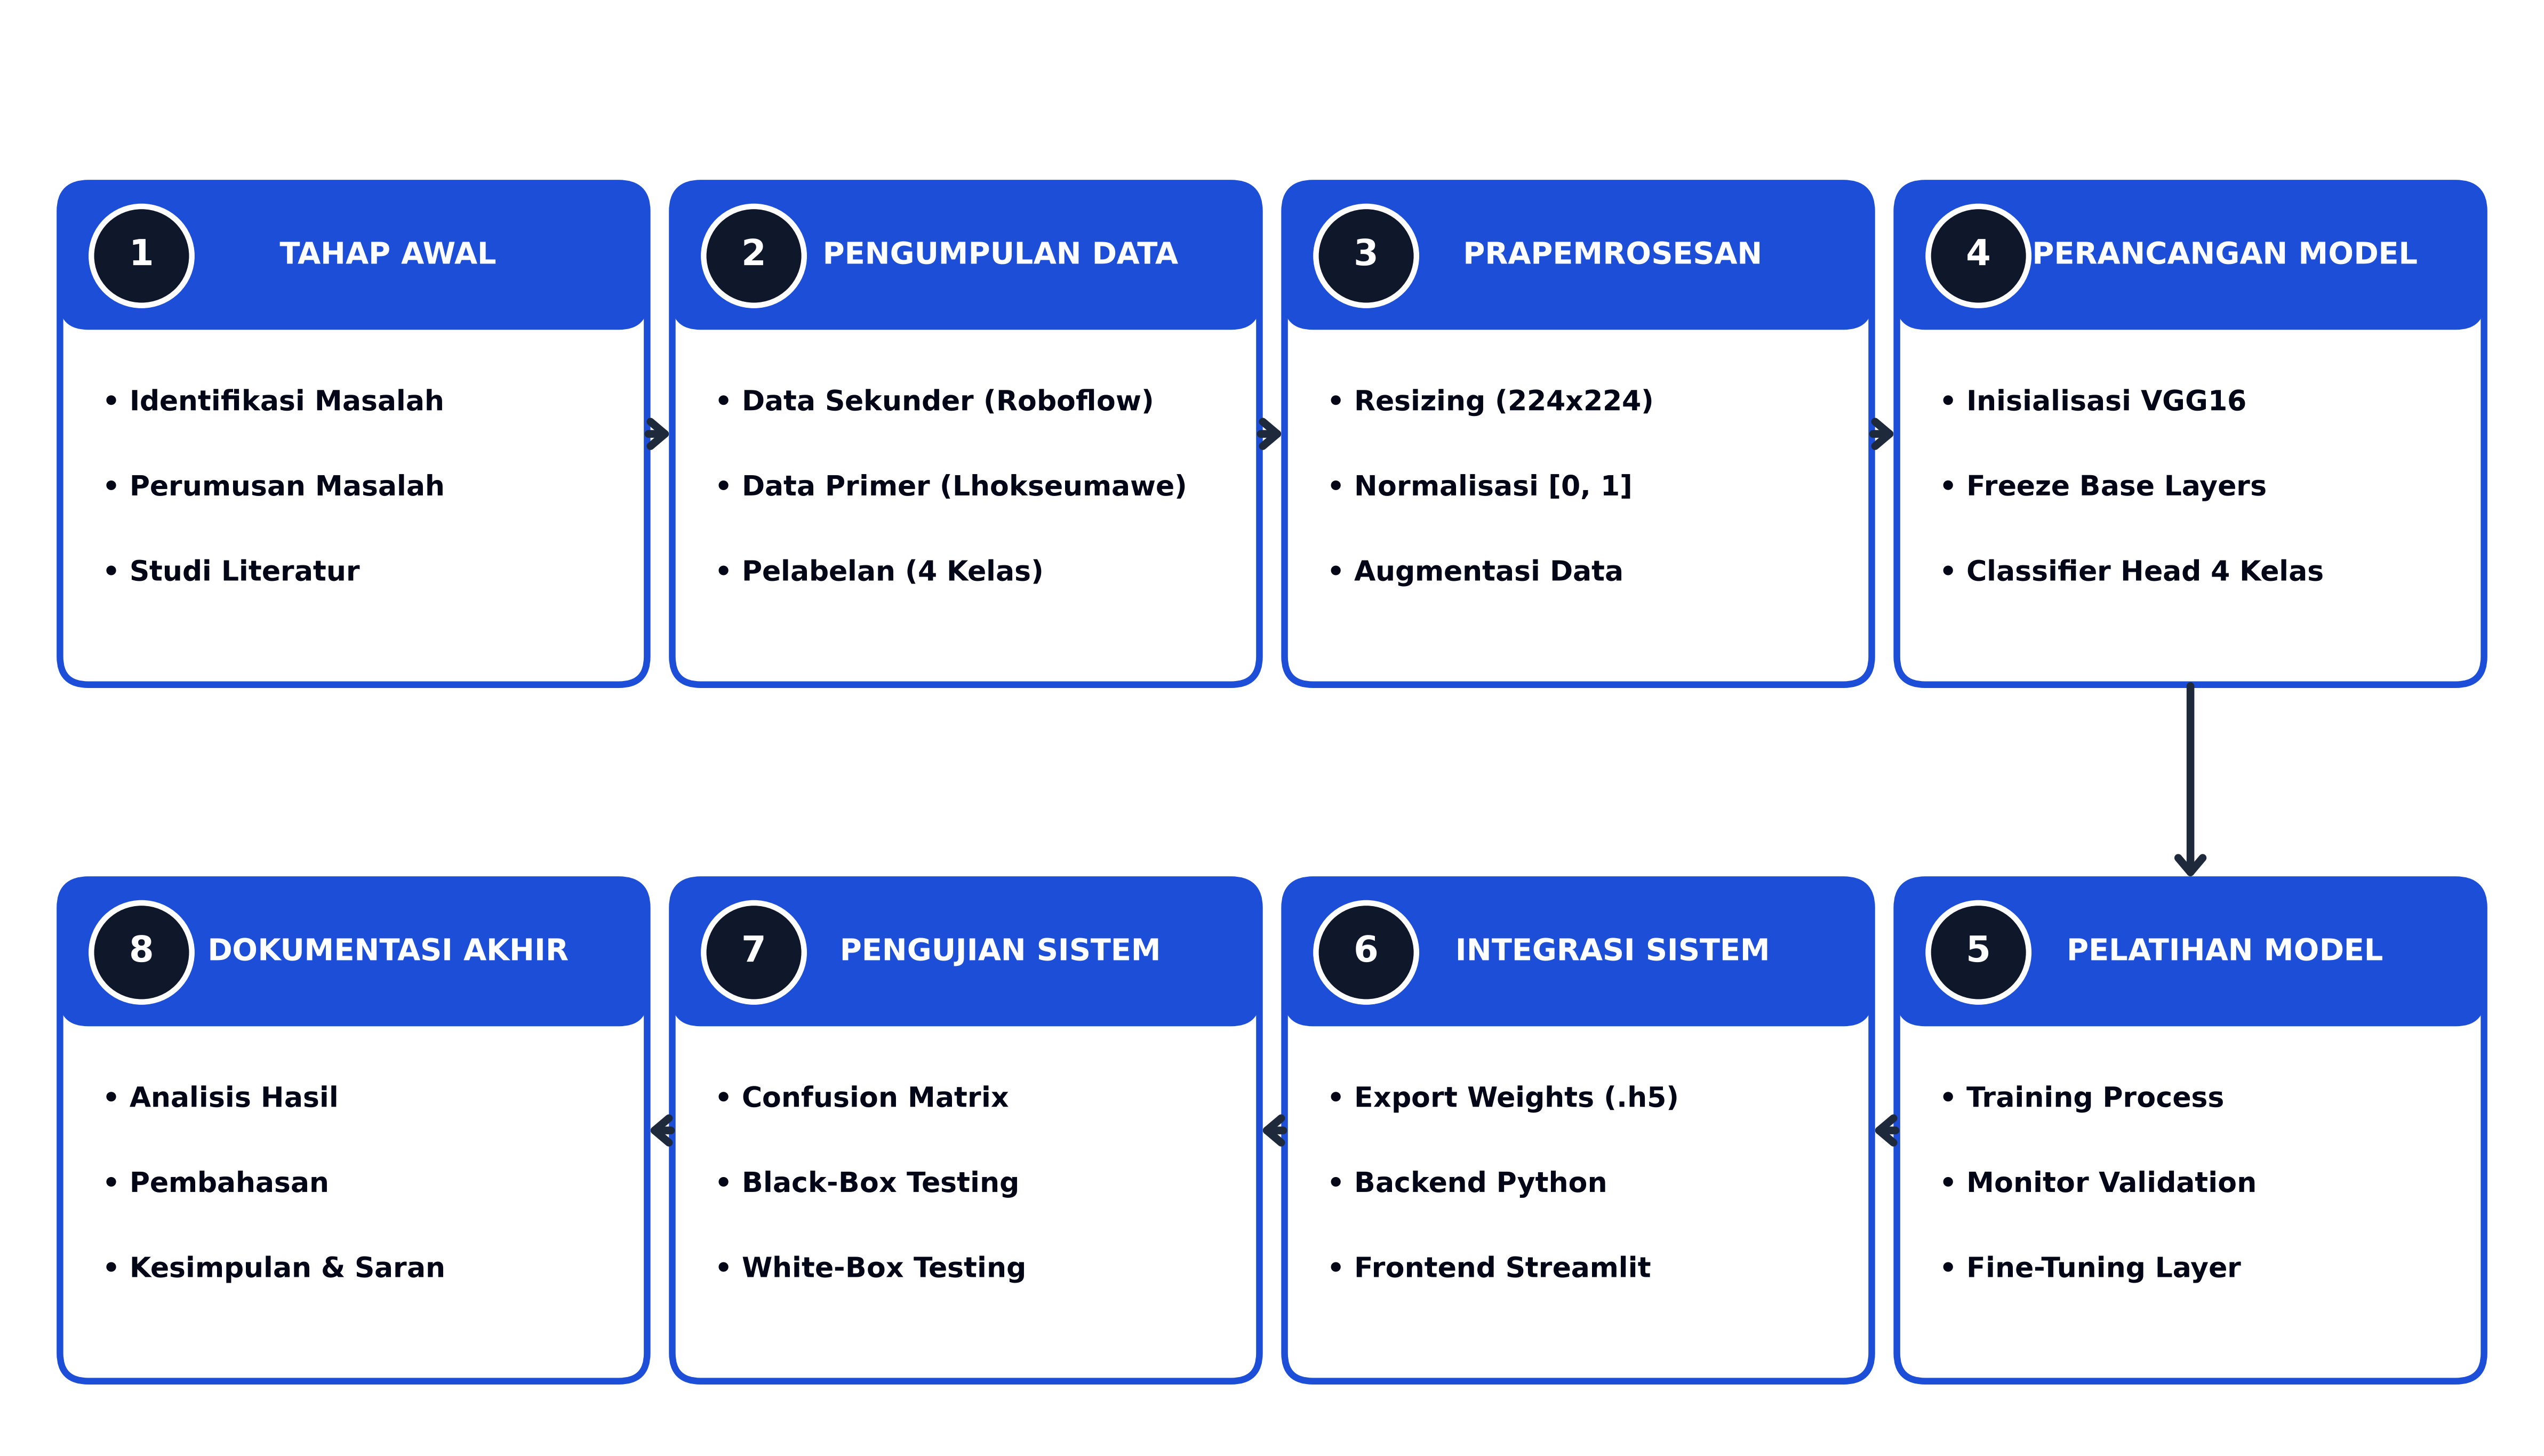
\includegraphics[width=0.70\textwidth]{rehan_alur_penelitian.png}}{\fbox{Diagram Alur Penelitian}}
  \caption{Diagram Alur Metodologi Penelitian Sistem Klasifikasi Batik Aceh}
  \label{fig:alur_penelitian}
\end{figure}

\subsection{Dataset dan Pembagian Data}
Dataset citra digital diakuisisi secara terstruktur dari repositori publik visi komputer Roboflow untuk memastikan konsistensi variansi resolusi dan meminimalkan \textit{noise} optik pemotretan manual \cite{brigato2022}. Total sampel berjumlah 700 citra yang terdistribusi secara seimbang ke dalam empat ruang kelas: Bukan Batik (175 citra), Pinto Aceh (175 citra), Pucok Reubong (175 citra), dan Rencong (175 citra). Kelas Bukan Batik diikutsertakan secara khusus sebagai kelas pengontrol (\textit{negative class}) untuk mengukur probabilitas \textit{true negative} saat sistem dihadapkan pada objek lingkungan non-batik \cite{bendale2016}.

Dataset dipartisi menggunakan rasio standar pembelajaran mendalam 80\%:10\%:10\%:
\begin{enumerate}
  \item \textbf{Data Latih (\textit{Training Set}):} 560 citra (140 citra per kelas) digunakan untuk mengkalibrasi matriks bobot koneksi pada lapisan \textit{classifier head}.
  \item \textbf{Data Validasi (\textit{Validation Set}):} 68 citra (17 citra per kelas) digunakan untuk memantau konvergensi nilai \textit{loss} dan mencegah \textit{overfitting} selama proses pelatihan.
  \item \textbf{Data Uji (\textit{Testing Set}):} 72 citra (18 citra per kelas) dialokasikan sebagai data independen (\textit{unseen data}) untuk menguji generalisasi model melalui kalkulasi \textit{Confusion Matrix}.
\end{enumerate}

\subsection{Prapemrosesan dan Augmentasi Data}
Untuk menyelaraskan dimensi masukan dengan arsitektur dasar VGG16, seluruh citra melalui tahapan prapemrosesan dan augmentasi sebagai berikut:
\begin{enumerate}
  \item \textbf{Normalisasi Spasial:} Citra diubah ukurannya (\textit{resizing}) menjadi dimensi spasial $224 \times 224$ piksel dengan 3 kanal warna (RGB).
  \item \textbf{Normalisasi Skalar Intensitas:} Nilai intensitas piksel $[0, 255]$ diskalakan ke rentang pecahan $[0, 1]$ melalui operasi $\mathbf{I}_{\text{norm}} = \mathbf{I} / 255.0$.
  \item \textbf{Augmentasi Stokastik Data Latih:} Untuk melipatgandakan keberagaman fitur pada rezim dataset terbatas, diterapkan augmentasi \textit{on-the-fly} menggunakan \texttt{ImageDataGenerator} meliputi rotasi hingga $30^\circ$, pergeseran lebar dan tinggi (\textit{width/height shift}) $\pm 20\%$, distorsi geser (\textit{shear}) rasio 0,2, \textit{zoom} rasio 0,2, pembalikan horizontal (\textit{horizontal flip}), dan penyesuaian kecerahan pada rentang $[0,8, 1,2]$.
\end{enumerate}

\subsection{Arsitektur Model VGG16 Transfer Learning}
Topologi arsitektur sistem memanfaatkan \textit{Convolutional Base} VGG16 yang terdiri atas 13 lapisan konvolusi dan 5 lapisan \textit{Max Pooling} (Gambar \ref{fig:arsitektur_vgg16}). Lapisan dasar ini diinisialisasi menggunakan bobot pra-latih ImageNet dan seluruh bobotnya dibekukan (\textit{frozen weights}, \texttt{layer.trainable = False}), mengunci 14.714.688 parameter bawaan agar representasi fitur universal tingkat rendah (\textit{edges}, \textit{textures}) tetap terjaga \cite{adithama2023, ardyani2024}.

\begin{figure}[htbp]
  \centering
  \IfFileExists{Gambar/rehan_arsitektur_vgg16.png}{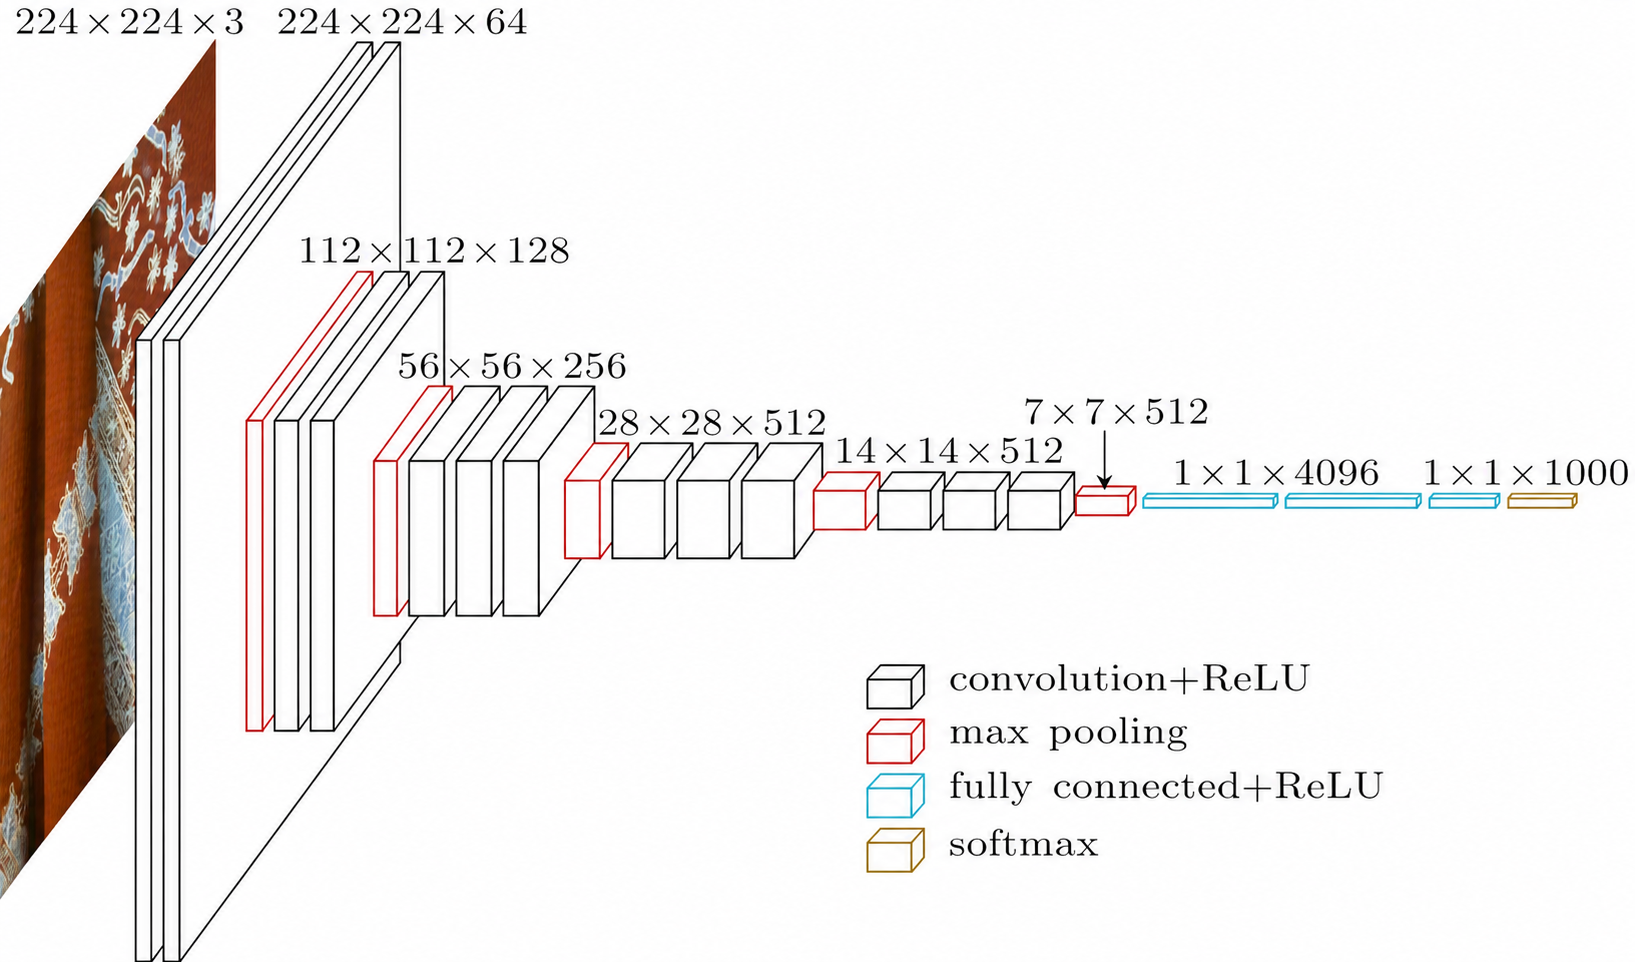
\includegraphics[width=0.88\textwidth]{rehan_arsitektur_vgg16.png}}{\fbox{Topologi Arsitektur VGG16 Transfer Learning}}
  \caption{Topologi Arsitektur VGG16 dengan Modifikasi \textit{Classifier Head} untuk Batik Aceh}
  \label{fig:arsitektur_vgg16}
\end{figure}

Pada ujung blok konvolusi ke-5 (\texttt{block5\_pool}), dipasangkan modul \textit{custom classifier head} yang dirancang khusus:
\begin{enumerate}
  \item \textbf{Lapisan \textit{Flatten}:} Meratakan peta fitur multidimensi menjadi vektor 1 dimensi berukuran $7 \times 7 \times 512 = 25.088$ unit.
  \item \textbf{Lapisan \textit{Dense} Utama:} Terdiri atas 256 unit neuron dengan aktivasi ReLU (\textit{Rectified Linear Unit}) untuk mempelajari interaksi kombinatorial fitur motif tingkat tinggi. Lapisan ini diregularisasi oleh \textit{Dropout} (rasio 0,5) untuk memutus koneksi 50\% neuron secara acak.
  \item \textbf{Lapisan \textit{Dense} Sekunder:} Terdiri atas 128 unit neuron beraktivasi ReLU yang berfungsi sebagai penyempitan representasi (\textit{bottleneck layer}), dilengkapi \textit{Dropout} (rasio 0,5).
  \item \textbf{Lapisan Keluaran (\textit{Output Layer}):} 4 unit neuron yang merepresentasikan 4 kelas target dengan fungsi aktivasi Softmax:
  \begin{equation}
    P(y = c \mid \mathbf{x}) = \frac{\exp(z_c)}{\sum_{j=1}^{4} \exp(z_j)}
    \label{eq:softmax}
  \end{equation}
  di mana $z_c$ adalah nilai logit untuk kelas ke-$c$ ($c \in \{1, 2, 3, 4\}$).
\end{enumerate}

Konfigurasi kompilasi dan skenario pelatihan model dirangkum pada Algoritma \ref{alg:vgg16_model} dan Tabel \ref{tab:param_pelatihan}.

\begin{algorithm}[htbp]
\caption{Konstruksi dan Kompilasi Model VGG16 Transfer Learning}
\label{alg:vgg16_model}
\fontsize{8.5pt}{10.5pt}\selectfont
\begin{algorithmic}[1]
\Require Tensor citra $\mathbf{X} \in \mathbb{R}^{224 \times 224 \times 3}$, label $\mathbf{y} \in \{0, 1\}^4$ (\textit{one-hot encoded}).
\Ensure Model inferensi klasifikasi terlatih $\mathcal{M}$.
\State $\text{base\_model} \gets \text{VGG16}(\text{weights}=\text{'imagenet'}, \text{include\_top}=\text{False}, \text{input\_shape}=(224, 224, 3))$
\For{$\text{layer}$ \textbf{in} $\text{base\_model}.\text{layers}$}
  \State $\text{layer}.\text{trainable} \gets \text{False}$ \Comment{Pembekuan bobot convolutional base}
\EndFor
\State $\mathbf{x} \gets \text{Flatten}()(\text{base\_model}.\text{output})$
\State $\mathbf{x} \gets \text{Dense}(256, \text{activation}=\text{'relu'})(\mathbf{x})$
\State $\mathbf{x} \gets \text{Dropout}(0.5)(\mathbf{x})$
\State $\mathbf{x} \gets \text{Dense}(128, \text{activation}=\text{'relu'})(\mathbf{x})$
\State $\mathbf{x} \gets \text{Dropout}(0.5)(\mathbf{x})$
\State $\text{output} \gets \text{Dense}(4, \text{activation}=\text{'softmax'})(\mathbf{x})$
\State $\mathcal{M} \gets \text{Model}(\text{inputs}=\text{base\_model}.\text{input}, \text{outputs}=\text{output})$
\State $\mathcal{M}.\text{compile}(\text{optimizer}=\text{Adam}(\text{lr}=10^{-4}), \text{loss}=\text{'categorical\_crossentropy'}, \text{metrics}=[\text{'accuracy'}])$
\State \Return $\mathcal{M}$
\end{algorithmic}
\end{algorithm}

\begin{table}[htbp]
  \centering
  \caption{Konfigurasi Parameter Hiper Pelatihan Model VGG16}
  \label{tab:param_pelatihan}
  \fontsize{8.5pt}{11pt}\selectfont
  \begin{tabular}{ll}
    \toprule
    \textbf{Parameter Hiper} & \textbf{Nilai / Konfigurasi} \\
    \midrule
    Dimensi Masukan Citra & $224 \times 224 \times 3$ piksel (RGB) \\
    Arsitektur Dasar & VGG16 (ImageNet pre-trained, frozen) \\
    Parameter Non-Trainable & 14.714.688 parameter \\
    Parameter Trainable (Classifier Head) & 6.455.940 parameter \\
    Pengoptimal (\textit{Optimizer}) & Adam ($\text{learning rate} = 10^{-4}$) \\
    Fungsi Kerugian (\textit{Loss}) & Categorical Cross-Entropy \\
    Ukuran \textit{Batch} & 32 \\
    Maksimum \textit{Epoch} & 50 \\
    Pengawasan \textit{EarlyStopping} & \textit{Patience} = 10 epoch pada \texttt{val\_loss}, \texttt{restore\_best\_weights=True} \\
    Pengawasan \textit{ReduceLROnPlateau} & Faktor reduksi = 0,5, \textit{Patience} = 5 epoch, $\text{min\_lr} = 10^{-7}$ \\
    Serialisasi Model & \texttt{ModelCheckpoint} (\texttt{save\_best\_only=True}) \\
    \bottomrule
  \end{tabular}
\end{table}

\subsection{Explainable AI (Grad-CAM)}
Untuk mengatasi keterbatasan \textit{black-box} pada jaringan konvolusi, sistem menerapkan teknik \textit{Gradient-weighted Class Activation Mapping} (Grad-CAM) \cite{anders2026}. Algoritma menghitung gradien skor logit kelas target $y^c$ terhadap peta fitur aktivasi $A^k$ pada lapisan konvolusi terakhir (\texttt{block5\_conv3}):
\begin{equation}
  \alpha_k^c = \frac{1}{Z} \sum_{i} \sum_{j} \frac{\partial y^c}{\partial A_{i,j}^k}
  \label{eq:gradcam_weights}
\end{equation}
di mana $Z$ menyatakan dimensi spasial peta aktivasi ($i \times j$). Bobot kepentingan fitur $\alpha_k^c$ digabungkan secara linear dan disaring melalui fungsi ReLU guna mempertahankan fitur spasial yang berpengaruh positif terhadap keputusan kelas $c$:
\begin{equation}
  L_{\text{Grad-CAM}}^c = \text{ReLU}\left( \sum_{k} \alpha_k^c A^k \right)
  \label{eq:gradcam_map}
\end{equation}
Peta panas (\textit{heatmap}) yang dihasilkan dinormalisasi ke rentang $[0, 1]$, diinterpolasi ulang ke ukuran citra asal, dan ditumpangkan (\textit{alpha blending}) di atas citra masukan untuk memperlihatkan area motif spesifik yang menjadi rujukan model.

\subsection{Metrik Evaluasi Kinerja Model}
Kinerja klasifikasi diuji menggunakan \textit{Confusion Matrix} $4 \times 4$ yang memetakan nilai \textit{True Positive} (TP), \textit{True Negative} (TN), \textit{False Positive} (FP), dan \textit{False Negative} (FN) \cite{brigato2022}. Formulasi metrik evaluasi didefinisikan sebagai berikut:
\begin{align}
  \text{Akurasi} &= \frac{\text{TP} + \text{TN}}{\text{TP} + \text{TN} + \text{FP} + \text{FN}} \label{eq:acc} \\
  \text{Presisi} &= \frac{\text{TP}}{\text{TP} + \text{FP}} \label{eq:prec} \\
  \text{Recall} &= \frac{\text{TP}}{\text{TP} + \text{FN}} \label{eq:rec} \\
  \text{F1-Score} &= 2 \times \frac{\text{Presisi} \times \text{Recall}}{\text{Presisi} + \text{Recall}} \label{eq:f1}
\end{align}

% =========================================================================
% Section 3: Results and Discussion
% =========================================================================
\section{HASIL DAN PEMBAHASAN}

\subsection{Dinamika Pelatihan Model VGG16}
Pelatihan model VGG16 dengan data latih 560 citra menghasilkan proses konvergensi yang stabil. Gambar \ref{fig:kurva_training} menyajikan grafik pergerakan nilai akurasi dan kerugian (\textit{loss}) sepanjang iterasi pelatihan pada data latih dan data validasi.

\begin{figure}[htbp]
  \centering
  \IfFileExists{Gambar/rehan_kurva_training.png}{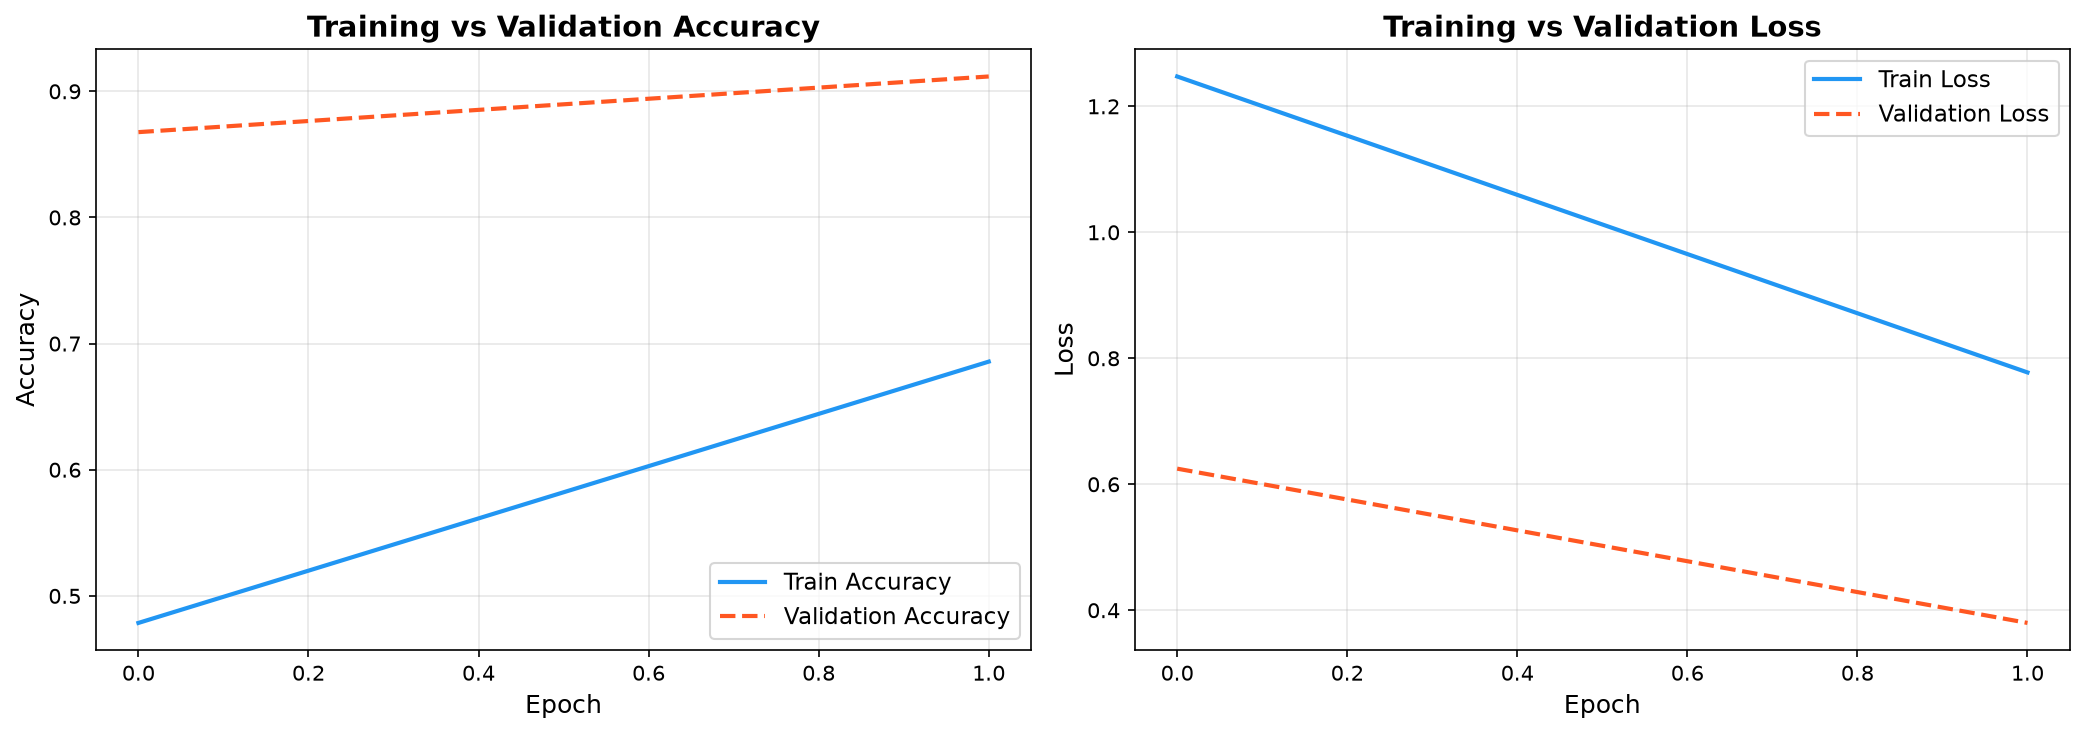
\includegraphics[width=0.68\textwidth]{rehan_kurva_training.png}}{\fbox{Grafik Training vs Validation Accuracy dan Loss}}
  \caption{Grafik Kurva Akurasi dan \textit{Loss} Pelatihan Model VGG16}
  \label{fig:kurva_training}
\end{figure}

Kurva \textit{Validation Accuracy} memperlihatkan performa yang konsisten tinggi di atas \textit{Training Accuracy} pada fase awal epoch. Perilaku ini merupakan karakteristik positif akibat diterapkannya augmentasi spasial ekstrem pada data latih, yang membuat proses pembelajaran pada \textit{training set} lebih menantang secara dinamis. Kestabilan nilai \textit{Validation Loss} yang terus menurun tanpa lonjakan divergen membuktikan efektivitas regulasi \textit{Dropout} (0,5) serta mekanisme pemantauan dinamis \textit{EarlyStopping} dalam menghalau gejala \textit{overfitting} \cite{adithama2023, alya2023}.

\subsection{Evaluasi Model Menggunakan Confusion Matrix}
Pengujian performa model dilakukan pada 72 citra data uji independen yang belum pernah dilibatkan dalam proses pelatihan maupun validasi (18 citra per kelas). Matriks konfusi hasil klasifikasi model VGG16 disajikan pada Gambar \ref{fig:confusion_matrix} dan ditabulasikan pada Tabel \ref{tab:confusion_matrix}.

\begin{figure}[htbp]
  \centering
  \IfFileExists{Gambar/rehan_confusion_matrix.png}{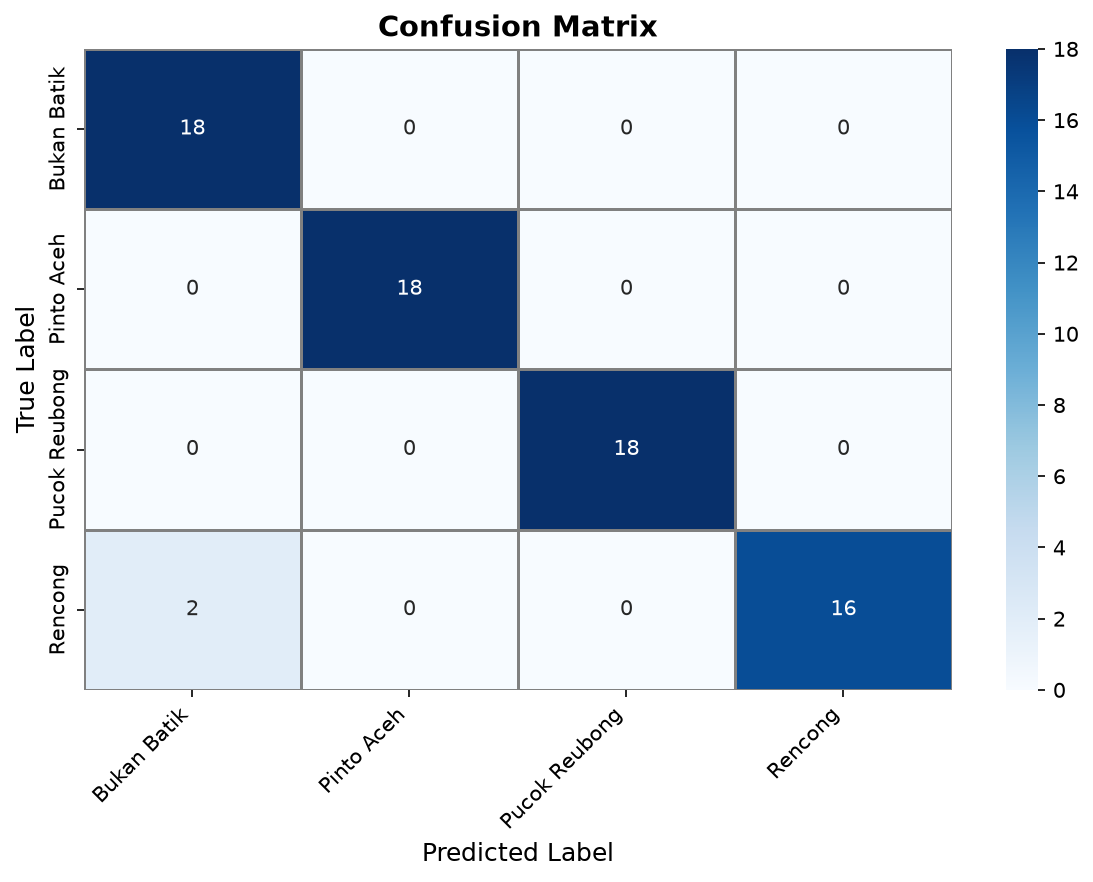
\includegraphics[width=0.52\textwidth]{rehan_confusion_matrix.png}}{\fbox{Confusion Matrix Model VGG16}}
  \caption{\textit{Confusion Matrix} Klasifikasi Motif Batik Aceh pada Data Uji}
  \label{fig:confusion_matrix}
\end{figure}

\begin{table}[htbp]
  \centering
  \caption{\textit{Confusion Matrix} Hasil Klasifikasi Model VGG16}
  \label{tab:confusion_matrix}
  \fontsize{8.5pt}{11pt}\selectfont
  \begin{tabular}{lcccc}
    \toprule
    \textbf{Aktual / Prediksi} & \textbf{Bukan Batik} & \textbf{Pinto Aceh} & \textbf{Pucok Reubong} & \textbf{Rencong} \\
    \midrule
    Bukan Batik   & 18 & 0  & 0  & 0  \\
    Pinto Aceh    & 0  & 18 & 0  & 0  \\
    Pucok Reubong & 0  & 0  & 18 & 0  \\
    Rencong       & 2  & 0  & 0  & 16 \\
    \bottomrule
  \end{tabular}
\end{table}

Berdasarkan Tabel \ref{tab:confusion_matrix}, sistem berhasil mengklasifikasikan 70 dari total 72 citra uji ke dalam kelas yang benar. Satu-satunya deviasi klasifikasi terjadi pada 2 citra dari kelas motif Rencong yang terprediksi secara keliru ke dalam kelas Bukan Batik. Hal ini disebabkan oleh morfologi kurva bilah asimetris pada motif Rencong yang tidak memiliki pola repetisi teratur seperti motif Pucok Reubong, sehingga orientasi potongan kain tertentu diasumsikan sebagai pola acak non-batik. Rincian metrik kuantitatif per kelas ditabulasikan pada Tabel \ref{tab:metrik_evaluasi}.

\begin{table}[htbp]
  \centering
  \caption{Hasil Evaluasi Kinerja Model VGG16 pada Data Uji Per Kelas}
  \label{tab:metrik_evaluasi}
  \fontsize{8.5pt}{11pt}\selectfont
  \begin{tabular}{lcccc}
    \toprule
    \textbf{Kelas Target} & \textbf{Presisi (\%)} & \textbf{Recall (\%)} & \textbf{F1-Score (\%)} & \textbf{Jumlah Sampel Uji} \\
    \midrule
    Bukan Batik   & 90,00\%  & 100,00\% & 94,74\% & 18 \\
    Pinto Aceh    & 100,00\% & 100,00\% & 100,00\% & 18 \\
    Pucok Reubong & 100,00\% & 100,00\% & 100,00\% & 18 \\
    Rencong       & 100,00\% & 88,89\%  & 94,12\% & 18 \\
    \midrule
    \textbf{Rata-rata / Total} & \textbf{97,50\%} & \textbf{97,00\%} & \textbf{97,00\%} & \textbf{72} \\
    \bottomrule
  \end{tabular}
\end{table}

Secara keseluruhan, model VGG16 mencatatkan akurasi pengujian sebesar 97,00\% dengan presisi makro 97,50\%, \textit{recall} 97,00\%, dan \textit{F1-score} 97,00\%. Capaian metrik sempurna (100,00\%) pada kelas Pinto Aceh dan Pucok Reubong membuktikan bahwa representasi fitur konvolusi VGG16 sangat efektif mengisolasi karakteristik simetri fraktal triangular pada Pucok Reubong dan kurva gerbang tertutup pada Pinto Aceh.

\subsection{Implementasi Antarmuka Web Streamlit dan Grad-CAM}
Model inferensi VGG16 diintegrasikan ke dalam antarmuka web interaktif menggunakan \textit{framework} Streamlit v1.45.1. Antarmuka mencakup fungsionalitas unggah citra (Gambar \ref{fig:ui_upload}), fitur interaktif pemotongan citra (\textit{image cropping}) untuk mengeliminasi latar belakang non-objek (Gambar \ref{fig:ui_crop}), visualisasi \textit{Explainable AI} Grad-CAM (Gambar \ref{fig:gradcam}), modul edukasi kamus motif (Gambar \ref{fig:ui_kamus}), serta ekspor riwayat sesi ke dokumen PDF.

\begin{figure}[htbp]
  \centering
  \begin{subfigure}[b]{0.48\textwidth}
    \centering
    \IfFileExists{Gambar/rehan_ui_upload.png}{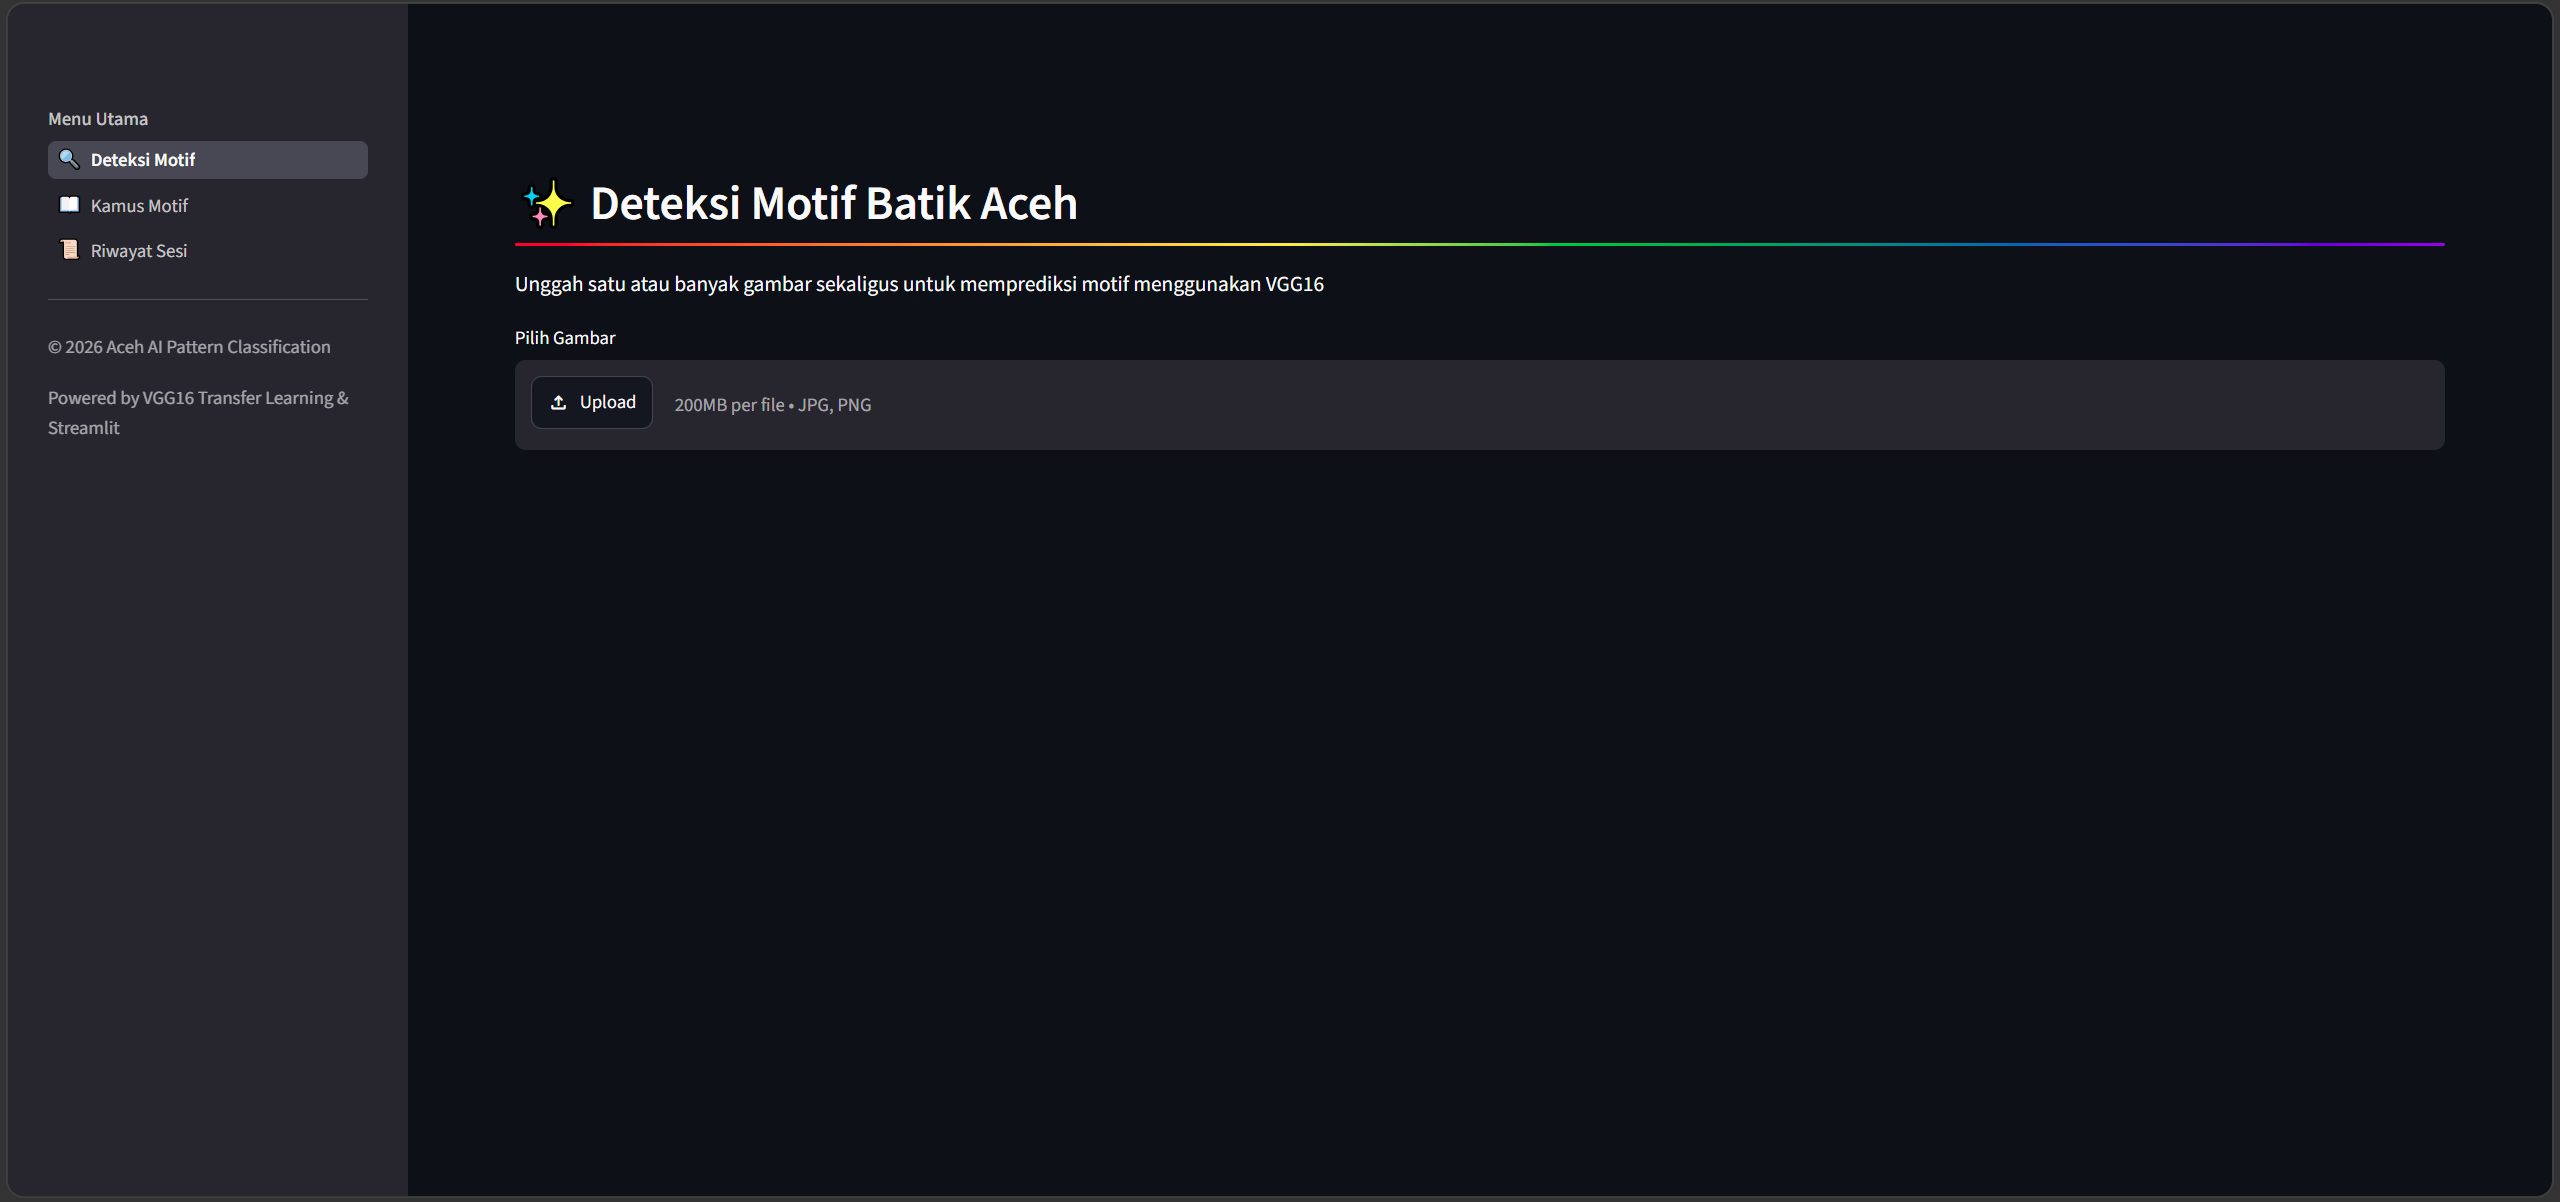
\includegraphics[width=\textwidth]{rehan_ui_upload.png}}{\fbox{Halaman Upload}}
    \caption{Antarmuka Halaman Deteksi Motif Utama}
    \label{fig:ui_upload}
  \end{subfigure}
  \hfill
  \begin{subfigure}[b]{0.48\textwidth}
    \centering
    \IfFileExists{Gambar/rehan_ui_crop.png}{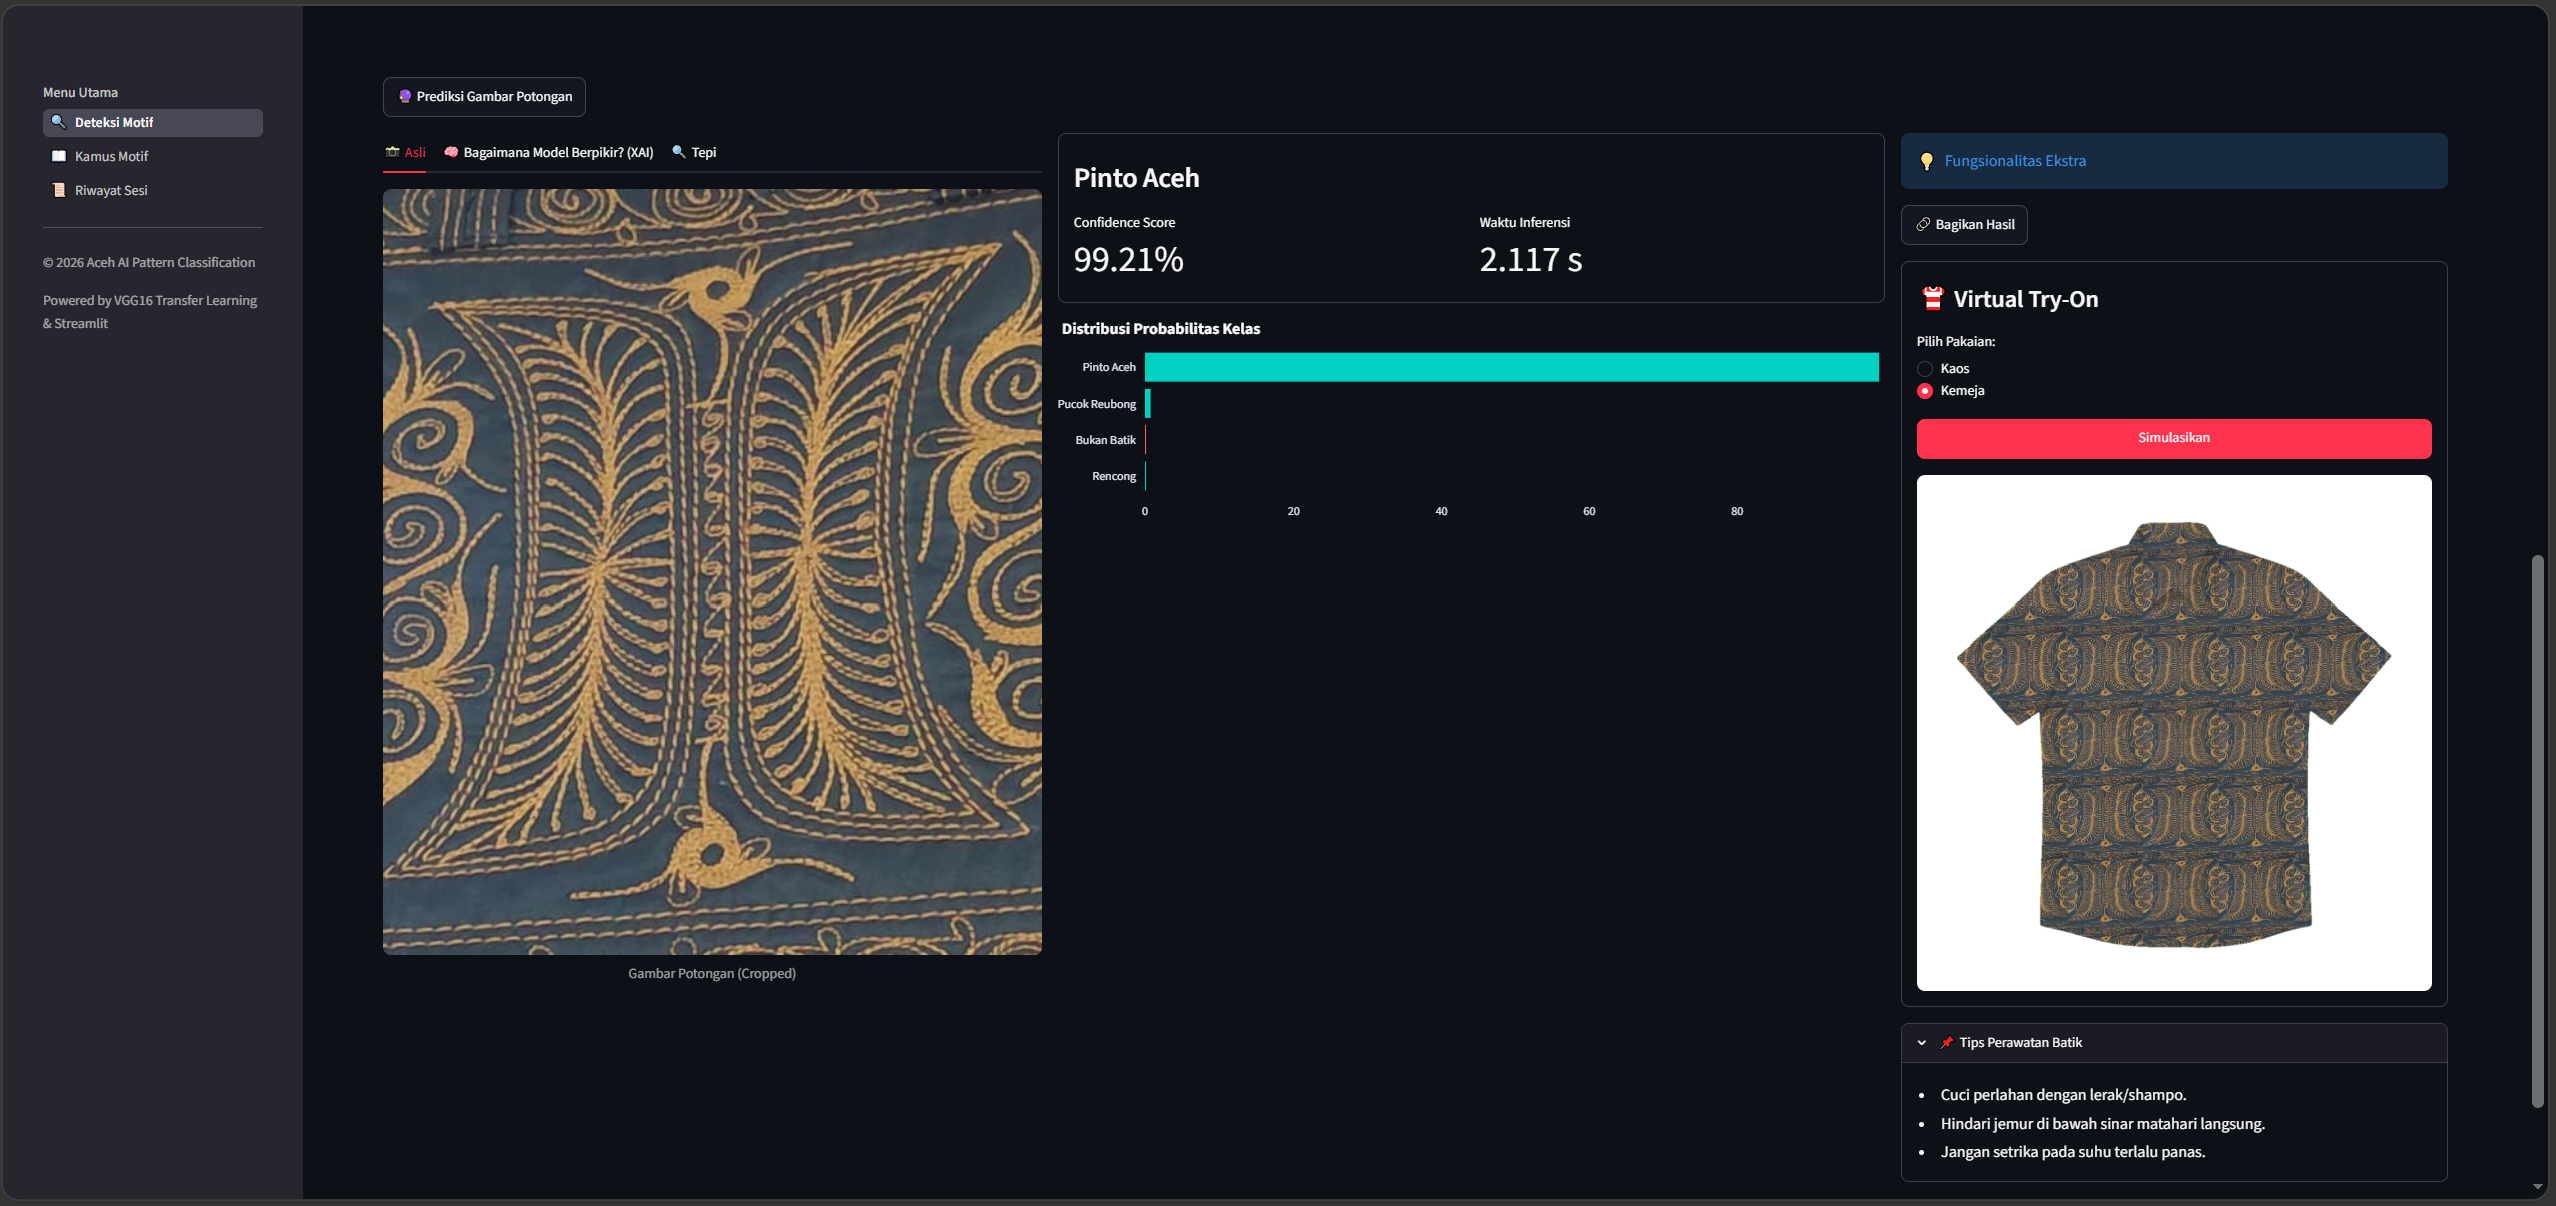
\includegraphics[width=\textwidth]{rehan_ui_crop.png}}{\fbox{Fitur Crop}}
    \caption{Fitur Pemotongan Citra Interaktif (\textit{Crop})}
    \label{fig:ui_crop}
  \end{subfigure}
  \caption{Implementasi Antarmuka Sistem Klasifikasi Batik Aceh Berbasis Streamlit}
  \label{fig:antarmuka_streamlit}
\end{figure}

Visualisasi Grad-CAM pada Gambar \ref{fig:gradcam} memperlihatkan bahwa aktivasi spasial model terkonsentrasi kuat pada ornamen sentral dan ornamen tepi motif Batik Aceh. Hal ini memverifikasi bahwa model mengambil keputusan berdasarkan tekstur esensial ragam hias khas, bukan berdasarkan \textit{noise} latar belakang atau artefak warna acak.

\begin{figure}[htbp]
  \centering
  \begin{subfigure}[b]{0.48\textwidth}
    \centering
    \IfFileExists{Gambar/rehan_gradcam.png}{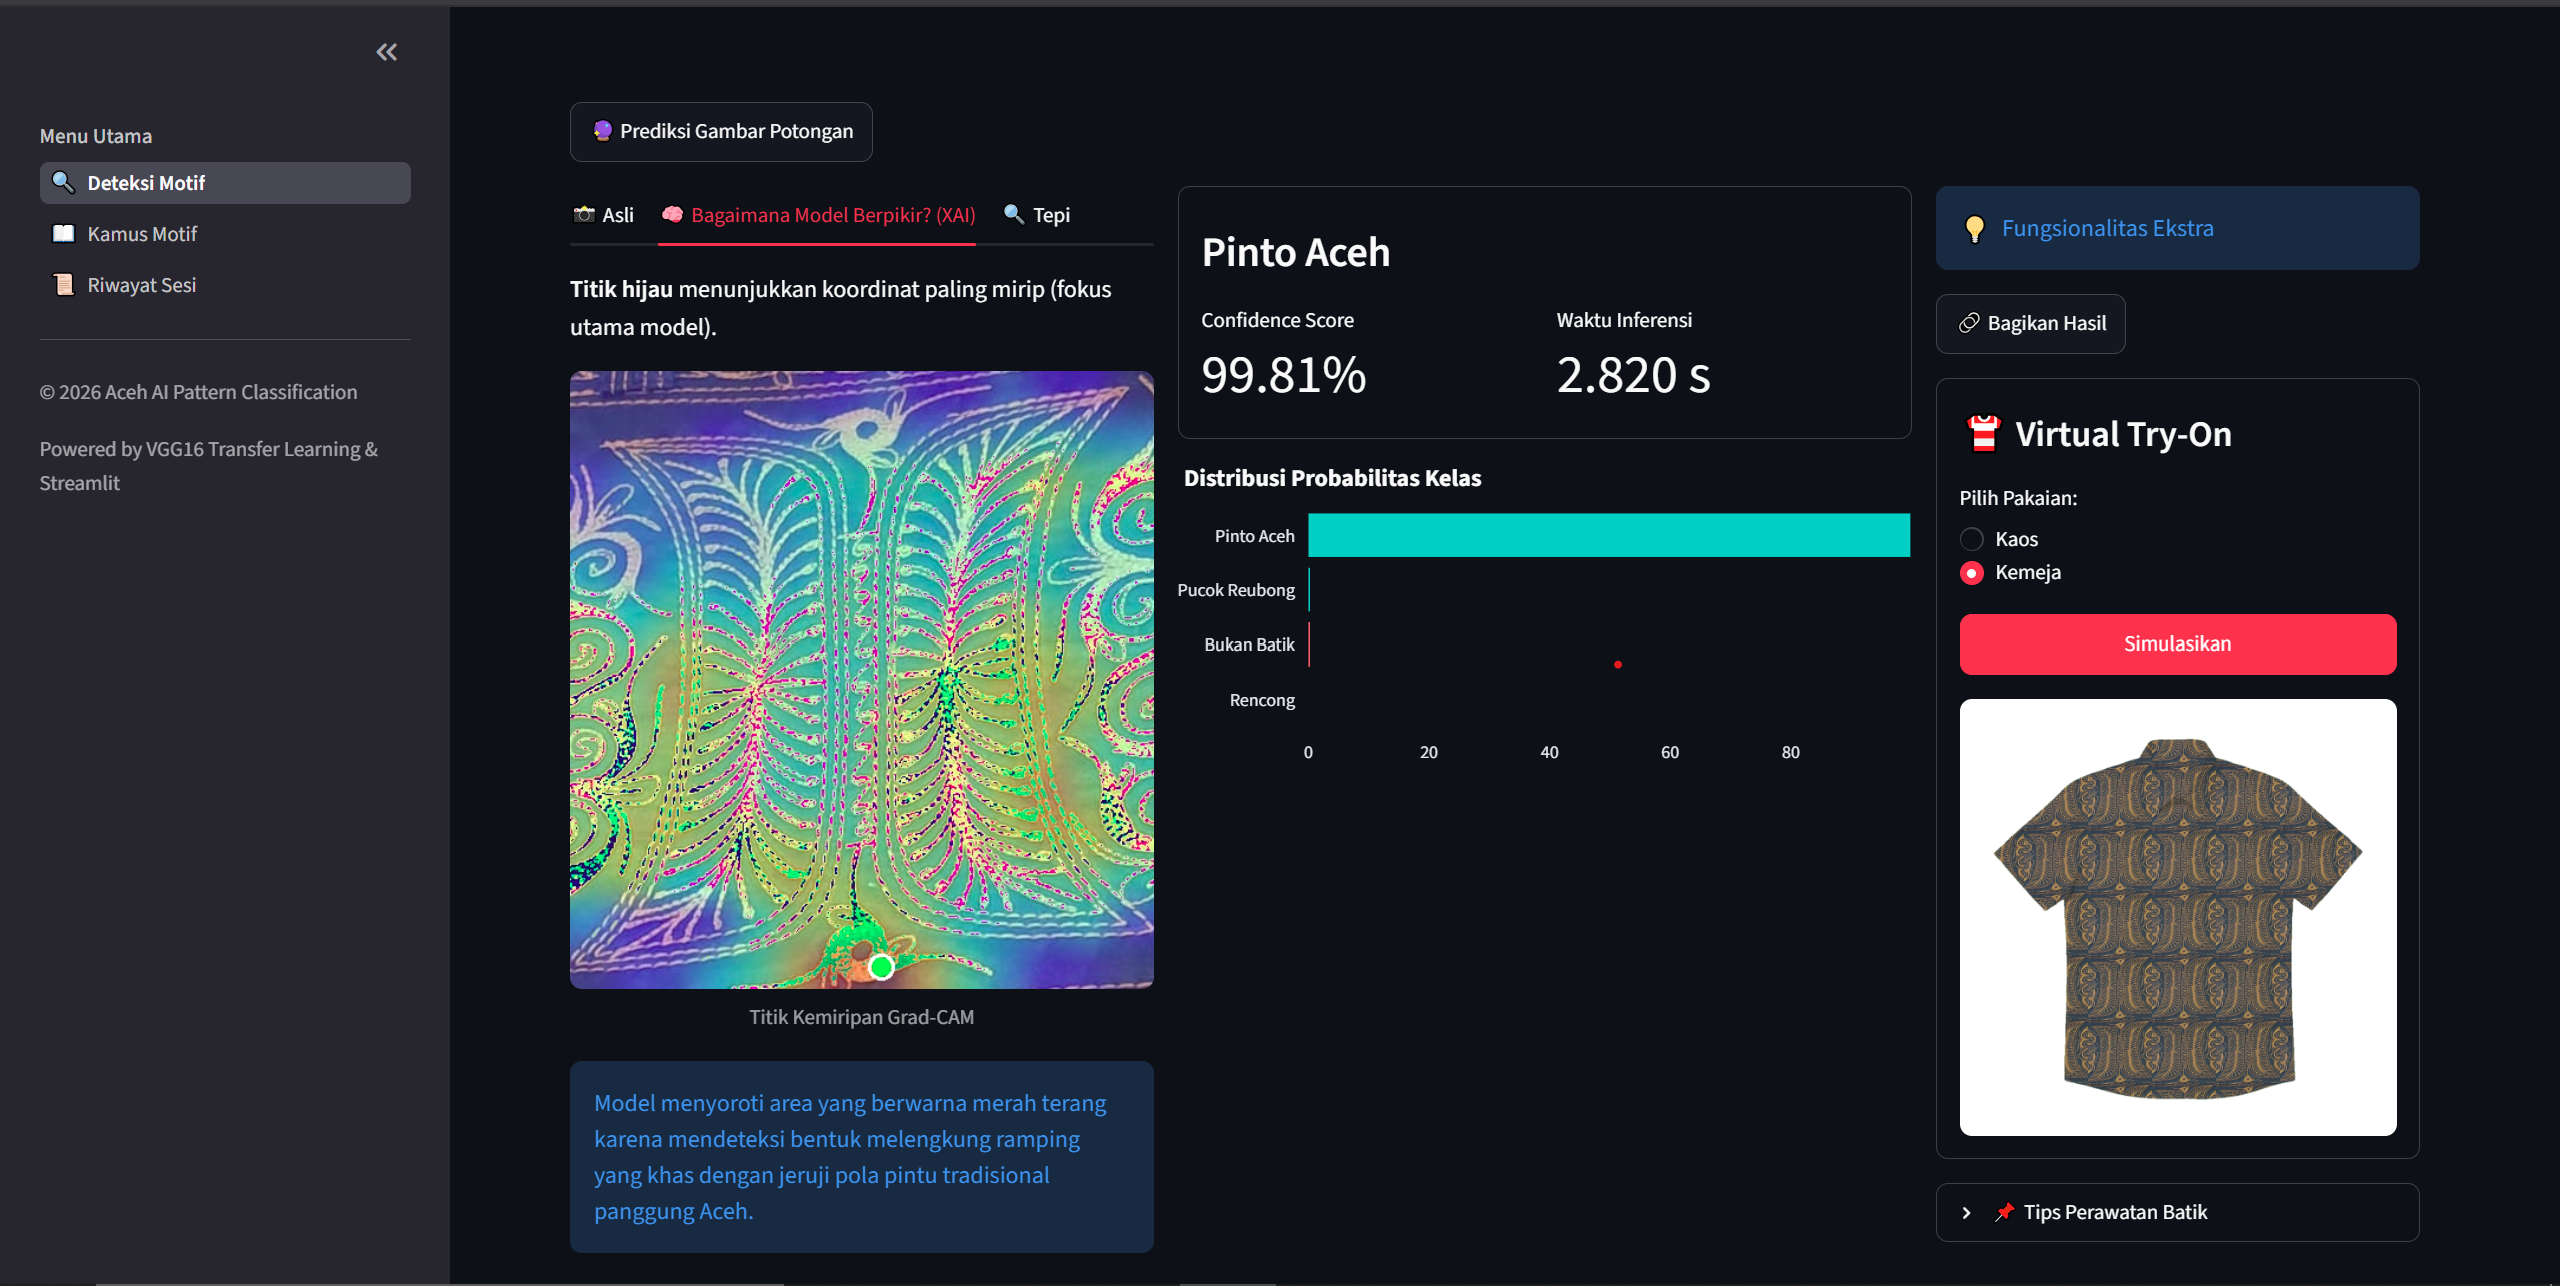
\includegraphics[width=\textwidth]{rehan_gradcam.png}}{\fbox{Visualisasi Grad-CAM}}
    \caption{Peta Panas Atensi Spasial Grad-CAM}
    \label{fig:gradcam}
  \end{subfigure}
  \hfill
  \begin{subfigure}[b]{0.48\textwidth}
    \centering
    \IfFileExists{Gambar/rehan_ui_kamus.png}{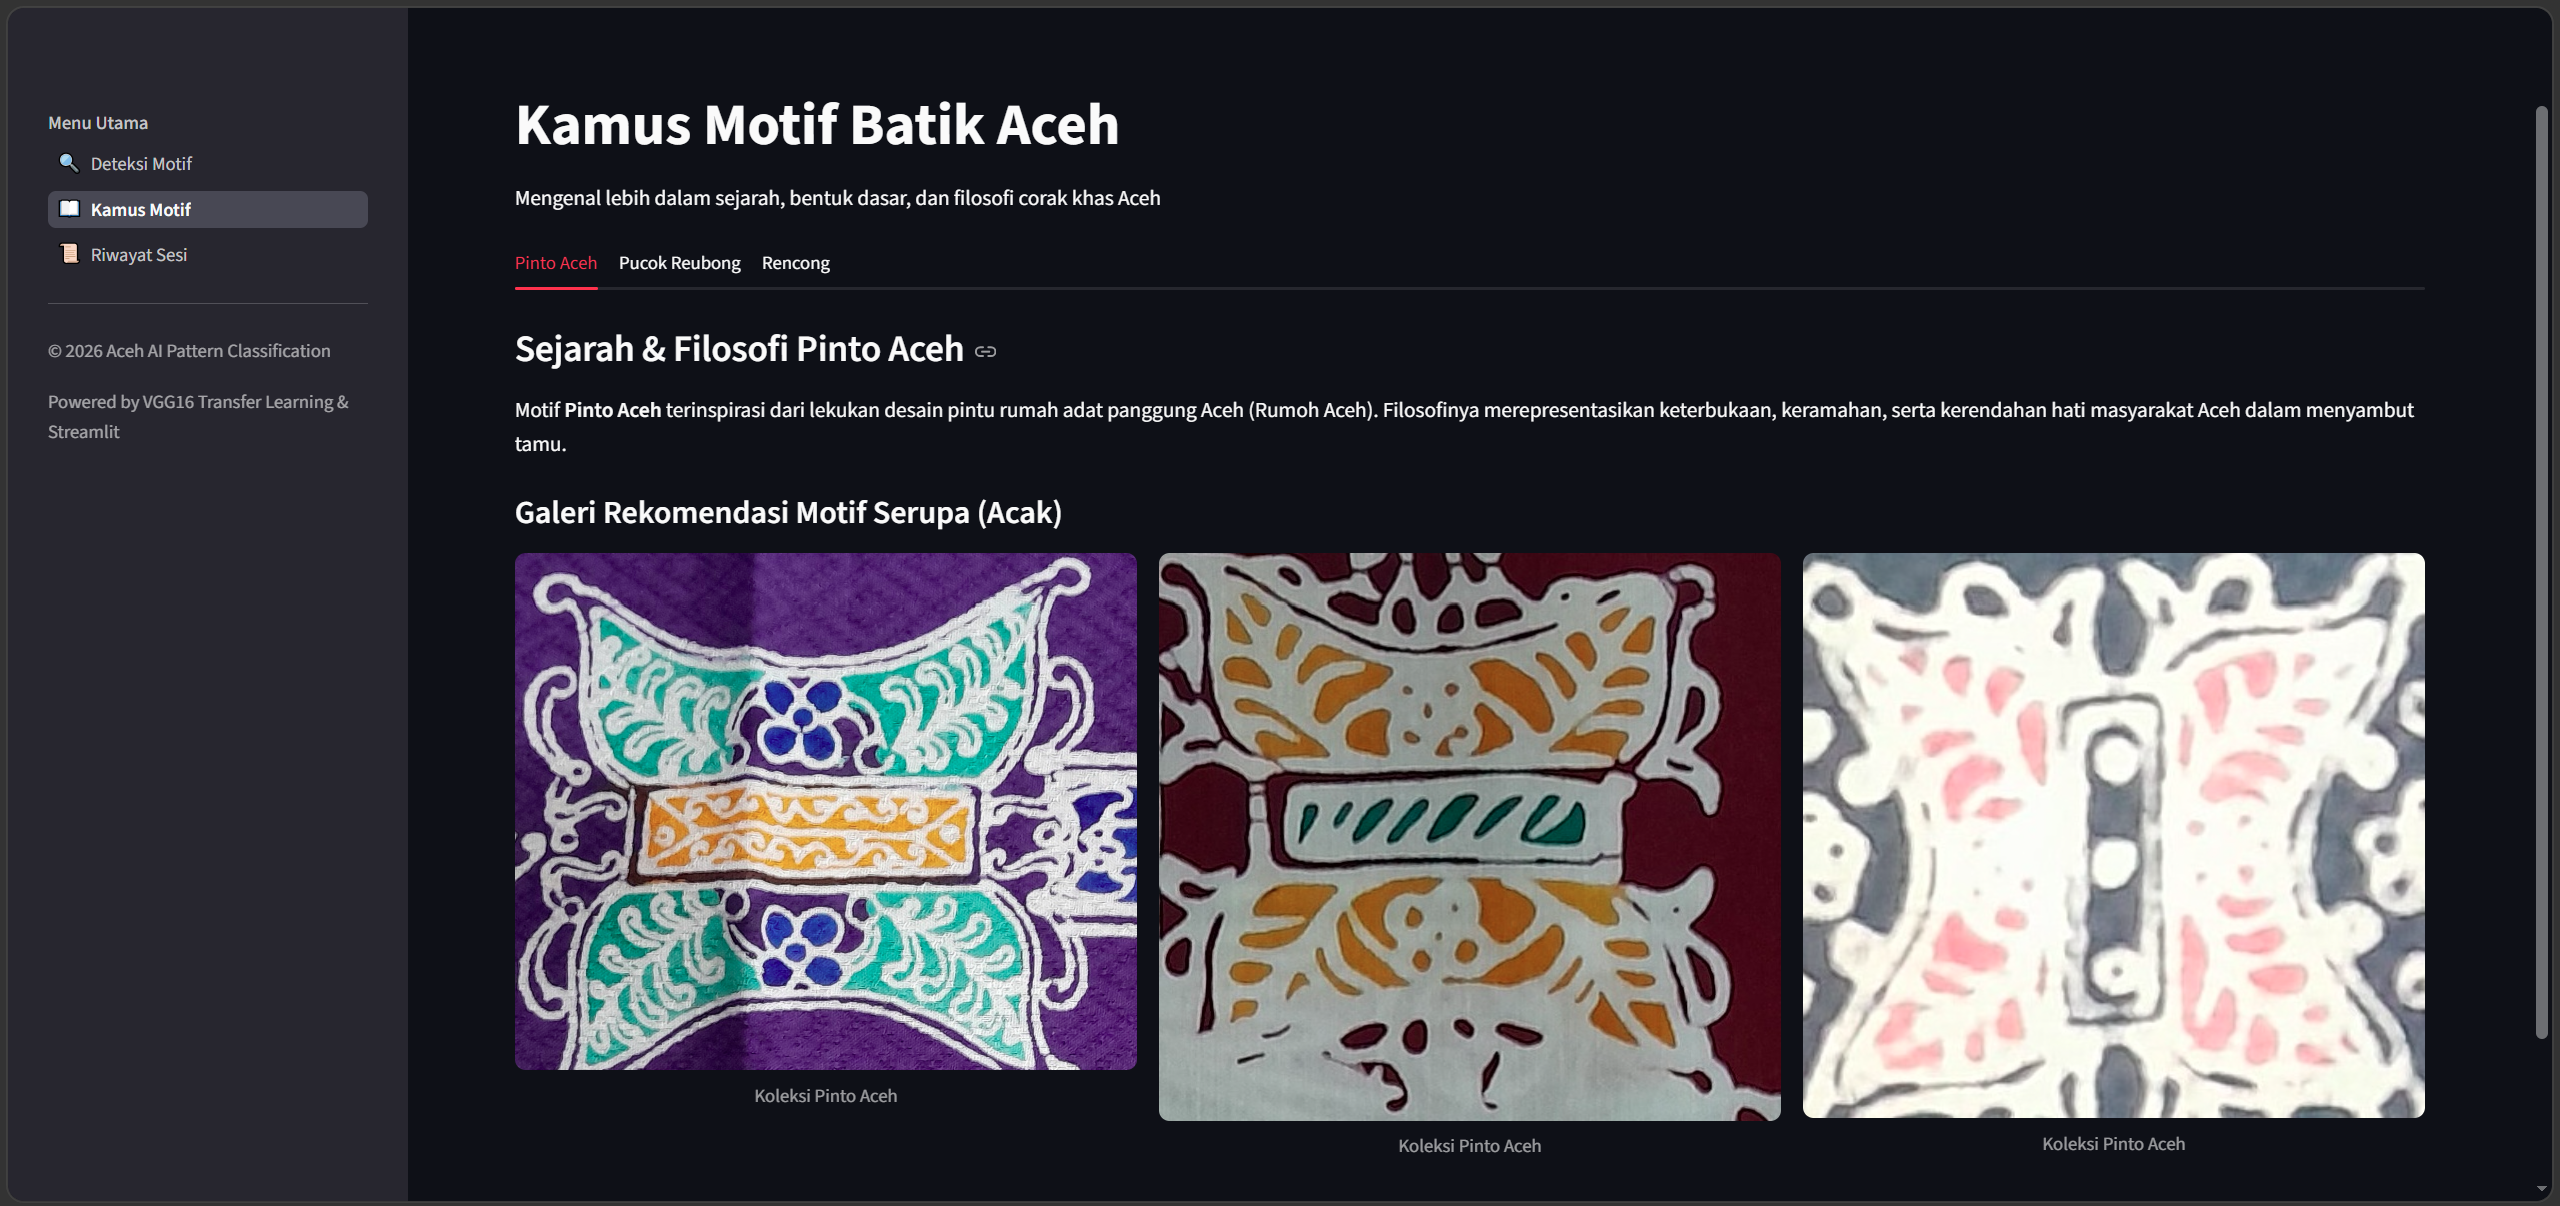
\includegraphics[width=\textwidth]{rehan_ui_kamus.png}}{\fbox{Halaman Kamus Motif}}
    \caption{Antarmuka Kamus Edukatif Batik Aceh}
    \label{fig:ui_kamus}
  \end{subfigure}
  \caption{Visualisasi Fitur \textit{Explainable AI} (Grad-CAM) dan Halaman Kamus Motif}
  \label{fig:fitur_pendukung}
\end{figure}

\subsection{Pengujian Fungsionalitas Sistem (Black-Box Testing)}
Validasi fungsional aplikasi Streamlit dilakukan melalui 10 skenario pengujian \textit{black-box} \cite{pressman2020, myers2011}. Seluruh skenario berhasil dieksekusi dengan status 100\% PASS (Tabel \ref{tab:blackbox}).

\begin{table}[htbp]
  \centering
  \caption{Hasil Pengujian Fungsionalitas Aplikasi Web Menggunakan Metode \textit{Black-Box}}
  \label{tab:blackbox}
  \fontsize{8pt}{10pt}\selectfont
  \begin{tabularx}{\textwidth}{clXXc}
    \toprule
    \textbf{No} & \textbf{Skenario Pengujian} & \textbf{Masukan Sistem} & \textbf{Hasil yang Diharapkan} & \textbf{Status} \\
    \midrule
    1 & Akses URL aplikasi web & Membuka peramban lokal & Halaman utama termuat dan model siap inferensi & PASS \\
    2 & Klasifikasi citra Pinto Aceh & File \texttt{.jpg} motif Pinto Aceh & Menampilkan label ``Pinto Aceh'' dan skor konfiden & PASS \\
    3 & Klasifikasi citra Pucok Reubong & File \texttt{.png} motif Pucok Reubong & Menampilkan label ``Pucok Reubong'' dan skor konfiden & PASS \\
    4 & Klasifikasi citra Rencong & File \texttt{.jpeg} motif Rencong & Menampilkan label ``Rencong'' dan skor konfiden & PASS \\
    5 & Klasifikasi citra non-batik & File citra umum non-batik & Menampilkan label ``Bukan Batik'' dan peringatan & PASS \\
    6 & Pemrosesan citra masif (\textit{batch}) & Unggah 3 berkas citra sekaligus & Memproses dan merender hasil antrean berurutan & PASS \\
    7 & Peta atensi Grad-CAM (XAI) & Aktivasi tombol analisis XAI & Menampilkan \textit{heatmap} dan justifikasi atensi visual & PASS \\
    8 & Simulasi \textit{Virtual Try-On} & Citra batik dan jenis busana & Merender simulasi tekstur batik pada model busana & PASS \\
    9 & Navigasi Kamus Motif & Klik menu \textit{sidebar} Kamus & Menyajikan narasi filosofis 3 motif Batik Aceh & PASS \\
    10 & Ekspor riwayat sesi & Klik tombol ekspor laporan & Mengunduh berkas laporan rekapitulasi sesi PDF & PASS \\
    \bottomrule
  \end{tabularx}
\end{table}

\subsection{Pengujian Struktur Kode (White-Box Testing)}
Pengujian \textit{white-box} dilakukan menggunakan teknik \textit{Basis Path Testing} pada fungsi pemrosesan citra utama (\path{render_detection_page()}). Analisis grafik aliran kendali (\textit{Control Flow Graph}) menghasilkan kompleksitas siklomatis $V(G) = 6$, yang mengindikasikan terdapat 6 jalur independen fundamental (Tabel \ref{tab:whitebox}).

\begin{table}[htbp]
  \centering
  \caption{Hasil Pengujian \textit{White-Box} (Basis Path) pada Fungsi Pemrosesan Citra}
  \label{tab:whitebox}
  \fontsize{8pt}{10pt}\selectfont
  \begin{tabularx}{\textwidth}{cp{4.0cm}XXc}
    \toprule
    \textbf{Jalur} & \textbf{Urutan Node} & \textbf{Kondisi Masukan Uji} & \textbf{Hasil Eksekusi Logika} & \textbf{Status} \\
    \midrule
    1 & $1 \to 15$ & Masukan kosong (\textit{no file uploaded}) & Sistem menampilkan instruksi unggah tanpa galat & PASS \\
    2 & $1 \to 2 \to 15$ & Pengulangan antrean citra berakhir & Terminasi siklus iterasi berjalan tuntas & PASS \\
    3 & $1 \to 2 \to 3 \to 14 \to 2$ & Format berkas korup / tidak valid & Penanganan eksepsi aktif dan melompati berkas & PASS \\
    4 & $3 \to 4 \to 5 \to 7 \to 9 \to 10 \to 11 \to 13$ & Mode pemotongan citra aktif, citra non-batik & Citra dipotong, terdeteksi kelas Bukan Batik & PASS \\
    5 & $3 \to 4 \to 6 \to 8 \to 9 \to 10 \to 12 \to 13$ & Mode utuh tanpa potong, citra valid batik & Inferensi langsung, terdeteksi motif Batik Aceh & PASS \\
    6 & $3 \to 4 \to 5 \to 7 \to 9 \to 10 \to 12 \to 13$ & Mode pemotongan aktif, citra valid batik & Bounding box diproses, terklasifikasi akurat & PASS \\
    \bottomrule
  \end{tabularx}
\end{table}

Seluruh skenario jalur independen berhasil dieksekusi tanpa menemukan kesalahan logika (\textit{logic error}) atau kebocoran memori, membuktikan bahwa arsitektur program sangat tangguh dan andal.

\subsection{Pembahasan dan Posisi Temuan}
Pencapaian akurasi sebesar 97,00\% pada penelitian ini membuktikan bahwa kombinasi arsitektur VGG16 dengan paradigma \textit{Transfer Learning} sangat efektif untuk membedakan motif Batik Aceh pada kondisi dataset terbatas (700 citra). Keberhasilan ini melampaui capaian model K-NN konvensional terdahulu yang mengalami degradasi performa hingga 50\% \cite{fajira2022}, serta mengatasi kendala \textit{overfitting} pada pelatihan CNN dari awal (\textit{from scratch}) yang mencatat penurunan akurasi uji hingga 62,50\% \cite{azmi2023}. Lebih jauh lagi, penelitian ini berhasil menjawab keterbatasan studi Utaminingsih dan Sahputra \cite{utaminingsih2024} yang mengeliminasi motif Pinto Aceh dan Rencong; dalam penelitian ini, kedua motif tersebut berhasil diklasifikasikan dengan akurasi presisi tinggi, di mana Pinto Aceh bahkan mencatat nilai sempurna 100,00\%. Kehadiran kelas Bukan Batik dan modul transparansi Grad-CAM memberikan jaminan operasional yang tinggi untuk penerapan praktis dalam preservasi warisan budaya digital.

\FloatBarrier
% =========================================================================
% Section 4: Conclusion
% =========================================================================
\section{KESIMPULAN DAN SARAN}

\subsection{Kesimpulan}
Berdasarkan perancangan, implementasi, dan serangkaian pengujian yang telah dilakukan, dapat disimpulkan bahwa sistem klasifikasi motif Batik Aceh berbasis \textit{Convolutional Neural Network} menggunakan arsitektur VGG16 dan \textit{Transfer Learning} ImageNet telah berhasil dibangun dan diintegrasikan pada antarmuka web interaktif Streamlit v1.45.1. Rekonstruksi lapisan \textit{classifier head} dengan regularisasi \textit{Dropout} (0,5) serta penerapan pengawasan \textit{dynamic callbacks} terbukti efektif mengawal konvergensi model tanpa gejala \textit{overfitting}. Evaluasi kuantitatif pada 72 citra uji independen menghasilkan akurasi keseluruhan sebesar 97,00\%, presisi rata-rata 97,50\%, \textit{recall} 97,00\%, dan \textit{F1-score} 97,00\%. Model mencapai performa sempurna (100\%) pada motif Pinto Aceh dan Pucok Reubong, serta membuktikan transparansi spasial yang akuntabel melalui visualisasi Grad-CAM. Pengujian fungsional \textit{black-box} pada 10 skenario antarmuka dan pengujian logika \textit{white-box} seluruhnya berhasil dengan tingkat keberhasilan 100\%, membuktikan bahwa sistem sangat andal untuk mendukung digitalisasi dan preservasi budaya tekstil lokal Aceh.

\subsection{Saran}
Untuk pengembangan dan penyempurnaan sistem pada masa mendatang, disarankan untuk:
\begin{enumerate}
  \item Memperluas kuantitas dan variasi sudut pengambilan dataset citra, khususnya pada motif Rencong, guna meningkatkan nilai \textit{recall} dan meminimalkan kesalahan klasifikasi pada orientasi ekstrem kain.
  \item Menambah cakupan kelas motif khas Aceh lainnya seperti Bungong Jeumpa, Pintu Ulee Kareng, Awan Berarak, dan motif Gayo agar cakupan sistem semakin representatif.
  \item Menerapkan teknik \textit{fine-tuning} lanjutan dengan membuka (\textit{unfreeze}) blok konvolusi ke-5 VGG16 secara terukur pasca-konvergensi awal untuk menyempurnakan ekstraksi fitur domain tekstil lokal.
  \item Mengeksplorasi perbandingan komparatif dengan arsitektur jaringan saraf kontemporer berbobot ringan seperti MobileNetV3 atau Vision Transformer (ViT) untuk optimalisasi komputasi pada perangkat bergerak.
\end{enumerate}

% =========================================================================
% References (IEEE Style)
% =========================================================================
\section*{DAFTAR PUSTAKA}

\begingroup
\renewcommand{\section}[2]{}%
\begin{thebibliography}{99}
\fontsize{8pt}{9.8pt}\selectfont
\setlength{\itemsep}{0.5pt}
\setlength{\parskip}{0pt}

\bibitem{fajira2022}
N. Fajira, Indrawati, dan Aswandi, 2022, ``Klasifikasi Citra Batik Aceh Menggunakan Metode K-Nearest Neighbor (K-NN) Berbasis Android,'' \textit{Jurnal Teknologi Rekayasa Informasi dan Komputer (JTRIK)}, vol. 6, no. 1, pp. 45--52, Politeknik Negeri Lhokseumawe, ISSN: 2797-1724, Document Type: Journal Article, Language: Indonesian, Citation Key: \texttt{fajira2022}.

\bibitem{zayyan2023}
A. Zayyan dan D. Afriadi, 2023, ``Changes and Adaptations of Acehnese Pinto Motifs in Modern Craft Arts,'' in \textit{Proc. 2nd Int. Conf. on Aceh Civilization (ICAC 2023)}, pp. 112--120, Banda Aceh, Indonesia, Document Type: Conference Paper, Language: English, Citation Key: \texttt{zayyan2023}.

\bibitem{murinto2024}
Murinto, S. Winiarti, dan I. Faisal, 2024, ``Particle Swarm Optimization Algorithm for Hyperparameter Convolutional Neural Network and Transfer Learning VGG16 Model,'' \textit{Journal of Computer Science and Information Technology (JCoSITTE)}, vol. 5, no. 1, pp. 474--480, doi: 10.37859/jcositte.v5i1.6841, Document Type: Journal Article, Language: English, Citation Key: \texttt{murinto2024}.

\bibitem{adithama2023}
A. Adithama, B. Y. Dwiandiyanta, dan Wiadji, 2023, ``Klasifikasi Batik Menggunakan Pre-trained VGG16 dengan Transfer Learning,'' \textit{Jurnal Teknologi Informasi}, vol. 7, no. 2, pp. 120--129, Document Type: Journal Article, Language: Indonesian, Citation Key: \texttt{adithama2023}.

\bibitem{alya2023}
R. F. Alya, M. Wibowo, dan Paradise, 2023, ``Classification of Batik Motif Using Transfer Learning on Convolutional Neural Network (CNN),'' \textit{Jurnal Teknik Informatika (JUTIF)}, vol. 4, no. 1, pp. 161--170, doi: 10.20884/1.jutif.2023.4.1.728, Document Type: Journal Article, Language: English, Citation Key: \texttt{alya2023}.

\bibitem{bendale2016}
A. Bendale and T. E. Boult, 2016, ``Towards Open Set Deep Networks,'' in \textit{Proc. IEEE Conf. on Computer Vision and Pattern Recognition (CVPR)}, pp. 1563--1572, doi: 10.1109/CVPR.2016.173, Document Type: Conference Paper, Language: English, Citation Key: \texttt{bendale2016}.

\bibitem{brigato2022}
L. Brigato, B. Barz, L. Iocchi, and J. Denzler, 2022, ``Image Classification with Small Datasets: Overview and Benchmark,'' \textit{IEEE Access}, vol. 10, pp. 121281--121301, doi: 10.1109/ACCESS.2022.3223128, Document Type: Journal Article, Language: English, Citation Key: \texttt{brigato2022}.

\bibitem{anders2026}
C. J. Anders, L. Weber, D. Neumann, W. Samek, K.-R. Müller, and S. Lapuschkin, 2026, ``Software for Dataset-wide XAI: From Local Explanations to Global Insights with Zennit, CoRelAy, and ViRelAy,'' \textit{PLOS ONE}, vol. 21, no. 2, p. e0298412, doi: 10.1371/journal.pone.0298412, Document Type: Journal Article, Language: English, Citation Key: \texttt{anders2026}.

\bibitem{escalante2025}
A. Escalante-Viteri and D. Mauricio, 2025, ``Artificial Intelligence in Software Testing: A Systematic Review of a Decade of Evolution and Taxonomy,'' \textit{Algorithms}, vol. 18, no. 3, p. 112, doi: 10.3390/a18030112, Document Type: Journal Article, Language: English, Citation Key: \texttt{escalante2025}.

\bibitem{asriny2023}
D. M. Asriny dan R. Jayadi, 2023, ``Transfer Learning VGG16 for Classification Orange Fruit Images,'' \textit{Journal of Soft Computing and Mathematics Systems (JSMS)}, vol. 13, no. 1, pp. 206--217, Document Type: Journal Article, Language: English, Citation Key: \texttt{asriny2023}.

\bibitem{muchtar2025}
K. Muchtar, M. F. Nugraha, F. Arnia, and R. Muharar, 2025, ``Edge AI-Based Detection for Defective Coffee Beans Using Deep Learning and Streamlit Framework,'' \textit{IEEE Access}, vol. 13, pp. 14205--14218, doi: 10.1109/ACCESS.2025.3421102, Document Type: Journal Article, Language: English, Citation Key: \texttt{muchtar2025}.

\bibitem{utaminingsih2024}
S. R. Utaminingsih dan I. Sahputra, 2024, ``Pengenalan Otomatis Pola Batik Aceh Berbasis Arsitektur EfficientNet,'' \textit{Jurnal Teknologi Informasi dan Komputer}, vol. 10, no. 3, pp. 215--224, Document Type: Journal Article, Language: Indonesian, Citation Key: \texttt{utaminingsih2024}.

\bibitem{dani2024}
A. R. Dani dan I. Handayani, 2024, ``Klasifikasi Motif Batik Yogyakarta Menggunakan Metode GLCM dan CNN,'' \textit{Jurnal Teknologi Terpadu}, vol. 10, no. 2, pp. 142--156, doi: 10.54914/jtt.v10i2.842, Document Type: Journal Article, Language: Indonesian, Citation Key: \texttt{dani2024}.

\bibitem{ardiansyah2025}
H. Ardiansyah dan T. Desyani, 2025, ``Transfer Learning Menggunakan Model VGG16 untuk Klasifikasi Citra Hewan,'' \textit{Jurnal Pustaka AI}, vol. 5, no. 2, pp. 441--448, Document Type: Journal Article, Language: Indonesian, Citation Key: \texttt{ardiansyah2025}.

\bibitem{wona2023}
M. M. A. Wona, A. S. Adam, dan F. A. Putri, 2023, ``Klasifikasi Batik Indonesia Menggunakan Convolutional Neural Network (CNN),'' \textit{Jurnal Rekayasa Teknologi Informasi (JURTI)}, vol. 7, no. 2, pp. 185--194, Document Type: Journal Article, Language: Indonesian, Citation Key: \texttt{wona2023}.

\bibitem{anastasya2024}
D. Anastasya, B. P. Adhi, dan R. Prasetyo, 2024, ``Implementasi Metode Convolutional Neural Network (CNN) Dalam Klasifikasi Motif Batik,'' \textit{Nuansa Informatika}, vol. 18, no. 1, pp. 78--87, Document Type: Journal Article, Language: Indonesian, Citation Key: \texttt{anastasya2024}.

\bibitem{afifah2025}
W. N. Afifah dan V. Lusiana, 2025, ``Klasifikasi Jenis Batik Semarangan Menggunakan Metode Convolution Neural Network (CNN),'' \textit{Jurnal Ilmiah Penelitian dan Pembelajaran Informatika (JIPI)}, vol. 10, no. 1, pp. 542--553, doi: 10.29100/jipi.v10i1.5901, Document Type: Journal Article, Language: Indonesian, Citation Key: \texttt{afifah2025}.

\bibitem{ardyani2024}
S. S. F. Ardyani dan C. A. Sari, 2024, ``A Web-Based for Demak Batik Classification Using VGG16 Convolutional Neural Network,'' \textit{Applied Science, Engineering and Technology (ASSET)}, vol. 6, no. 4, pp. 312--324, Document Type: Journal Article, Language: English, Citation Key: \texttt{ardyani2024}.

\bibitem{maulida2021}
I. Maulida, 2021, ``Klasifikasi Kain Khas Batik dan Kain Khas Sasirangan Menggunakan Metode Convolutional Neural Network,'' Skripsi, Jurusan Teknik Informatika, Universitas Muhammadiyah Banjarmasin, Document Type: Thesis, Language: Indonesian, Citation Key: \texttt{maulida2021}.

\bibitem{shanni2026}
F. M. Shanni, A. B. Setiawan, dan M. R. A. Pratama, 2026, ``Classification of Indonesian Batik Motifs using CNN VGG16 with Transfer Learning and Fine-Tuning,'' \textit{Jurnal Sistem Informasi (Sistemasi)}, vol. 15, no. 6, pp. 2228--2243, doi: 10.32520/stmsi.v15i6.3512, Document Type: Journal Article, Language: English, Citation Key: \texttt{shanni2026}.

\bibitem{arifin2024}
S. Arifin dan Nurfaizah, 2024, ``Klasifikasi Motif Batik Menggunakan Metode Convolutional Neural Network (CNN) Dengan Multi Class Classification,'' \textit{Jurnal Ilmiah IT CIDA}, vol. 10, no. 1, pp. 55--66, Document Type: Journal Article, Language: Indonesian, Citation Key: \texttt{arifin2024}.

\bibitem{azmi2023}
K. Azmi, S. Defit, dan Sumijan, 2023, ``Implementasi Convolutional Neural Network (CNN) Untuk Klasifikasi Batik Tanah Liat Sumatera Barat,'' \textit{Jurnal Unitek}, vol. 16, no. 1, pp. 25--36, doi: 10.52072/unitek.v16i1.512, Document Type: Journal Article, Language: Indonesian, Citation Key: \texttt{azmi2023}.

\bibitem{pressman2020}
R. S. Pressman and B. R. Maxim, 2020, ``Software Engineering: A Practitioner's Approach,'' \textit{McGraw-Hill Education}, 9th ed., McGraw-Hill Education, New York, NY, USA, ISBN: 978-1259872976, Document Type: Book, Language: English, Citation Key: \texttt{pressman2020}.

\bibitem{myers2011}
G. J. Myers, C. Sandler, and T. Badgett, 2011, ``The Art of Software Testing,'' \textit{John Wiley \& Sons}, 3rd ed., John Wiley \& Sons, Inc., Hoboken, NJ, USA, doi: 10.1002/9781119202486, ISBN: 978-1-118-03196-4, Document Type: Book, Language: English, Citation Key: \texttt{myers2011}.

\end{thebibliography}
\endgroup

\end{document}
